
\documentclass[submit]{ipsj}
%\documentclass{ipsj}

%\usepackage{graphicx}
%\usepackage[dvipdfmx]{graphicx,color}
%\usepackage[dvips]{graphicx}
\usepackage[dvipdfmx]{graphicx}
\usepackage{latexsym}
\usepackage{url}
\usepackage{listings}
\usepackage{multirow}


\newcommand{\todo}[1]{\colorbox{yellow}{{\bf TODO}:}{\color{red} {\textbf{[#1]}}}}


\def\Underline{\setbox0\hbox\bgroup\let\\\endUnderline}
\def\endUnderline{\vphantom{y}\egroup\smash{\underline{\box0}}\\}
\def\|{\verb|}

\setcounter{巻数}{59}
\setcounter{号数}{1}
\setcounter{page}{1}


\受付{2016}{3}{4}
\再受付{2015}{7}{16}   %省略可能
\再再受付{2015}{7}{20} %省略可能
\再再受付{2015}{11}{20} %省略可能
\採録{2016}{8}{1}




\begin{document}


\title{OSSリポジトリにおいて共変更関係を有するREADMEファイルとその他のファイルとの紐付け手法}

\etitle{A linkage approach of co-change relationship between README file and the other files in OSS repositories}

\affiliate{WA}{和歌山大学\\
Wakayama University, Sakaedani 930, Wakayama-city 640-8510, Japan}


% \paffiliate{WA}{和歌山大学\\
% Johoshori University}

\author{石岡 直樹}{Naoki Ishioka}{WA}[ishioka.naoki@g.wakayama-u.jp]
\author{伊原 彰紀}{Akinori Ihara}{WA}[ihara@wakayama-u.ac.jp]

\begin{abstract}
本論文では,開発者のREADME変更支援のために,同時に変更されるREADMEとその他ファイルの紐付け手法を提案した.分析1では,提案手法の性能を低下させる要因になる,ソースコードの変更とは無関係なREADMEのリファクタリングを目的とした変更が行われているのかを調査した.52,292件のREADMEを対象に,初期版と最終版のREADMEの項目と説明文を比較した結果,READMEの変更において,ソースコードの変更とは無関係なREADMEの変更が行われる可能性は低く,ソースコードの変更とともに項目ごとに情報を追加していくことを明らかにした.
分析2では,提案手法によってREADMEの変更とその他のファイルの変更を機械的に紐付けることができるのかを調査した.同時に変更されたREADMEの変更内容とファイルの変更内容を入力として,READMEとファイルの変更意図が一致するか否かの2クラス分類を行い,3つのモデル(BoW,BERT,CodeBERT)で比較した.その結果,CodeBERT(F1値=0.81),BoW(F1値=0.78),BERT(F1値=0.77)の順で高く,READMEとファイルの紐付けにおいて,CodeBERTモデルが適合率と再現率の両方で良好な性能を示した.
\end{abstract}


\begin{jkeyword}
README,ソフトウェアドキュメント,ソフトウェア工学,OSS開発
\end{jkeyword}

\begin{eabstract}
\todo{hoge}
\end{eabstract}

\begin{ekeyword}
\todo{hoge}
\end{ekeyword}

\maketitle

\section{はじめに}
%\textcolor{red}{henkoukasyo}

%RM変更の2種類説明
%RM変更をどのように支援するのか→紐づけ→リファクタリングみたいなやつは嫌→分析1でどのくらいあるか確認,分析2でモデル構築


オープンソースソフトウェア (OSS) は,プロジェクトの管理権を持っていない不特定多数の個人がプロジェクトに参加し,ソースコード修正やバグ報告,単に使用するなど様々な形で貢献している.多くのOSS開発プロジェクトは,ソフトウェアおよびプロジェクトに興味を持つ開発者の参加障壁を下げるために,ソースコードと併せてソフトウェアを説明するドキュメントを公開している.特に,GitHub\footnote[1]{https://github.com/}では,リポジトリ作成時にREADMEを作成することが推奨されている\footnote[2]{https://help.github.com/articles/about-readmes/}.READMEには,ソフトウェアを正しく利用するための情報(インストール方法,使用方法)や開発を促進するための情報(プロジェクトへの貢献方法)などが記述される.READMEはプロジェクトが所有するリポジトリのトップページに表示され,利用者や新規開発者にとって重要な役割を担っている\cite{Eco2011_Mens}.

% オープンソースソフトウェア (OSS) は,ソフトウェアの開発や配布において,ソースコードが一般に公開され,誰でも自由に利用,修正,拡張,再配布が可能なライセンスの元で提供されるソフトウェアの総称である\cite{Ikeda_7}.OSSでは,ソフトウェア開発プロジェクトのメンバー以外にも,
% プロジェクトに対して直接的な所有権や管理権を持っていない外部の個人や組織,つまり外部貢献者がプロジェクトに参加し,コード修正やバグ報告,テスト実行など様々な形でプロジェクトに貢献する.多くのOSS開発プロジェクトは,ソフトウェアおよびプロジェクトに興味を持つ外部の貢献者候補に向けて,ソースコードと併せてソフトウェアを説明するドキュメントを公開している.特に,GitHub~\footnote[1]{https://github.com/}では,プロジェクトを作成する際,最初にREADMEと呼ばれるドキュメントを作成することが推奨されている~\footnote[2]{https://help.github.com/articles/about-readmes/}.READMEには,ソフトウェアを正しく利用するための情報(インストール方法,使用方法)や開発を促進するための情報(プロジェクトへの貢献方法)などが記述される.READMEはプロジェクトが所有するリポジトリのトップページに表示され,利用者だけでなく新規開発者にとって重要な役割を担っている\cite{Kamei_7}.

プロジェクトの正しい情報を利用者や開発者に共有するために,ソフトウェアの進化に追従してREADMEを変更することが期待されるが,開発者にとってREADMEの作成や変更は多くの労力を要する\cite{Doc_maintenance1}\cite{Doc_maintenance2}.2017年に発表されたGitHubの調査結果~\footnote[3]{Open Source Survey: \url{https://opensourcesurvey.org/2017/}}では,開発者はREADMEを重要視している一方で,READMEの変更は頻繁に見落とされ,内容が不完全であったり,古いままになっていたりする問題を指摘している.READMEの変更は,ソースコードが変更に合わせて更新される場合と,ソースコードの変更とは無関係にREADMEの内部構造のリファクタリングのために更新する場合と2種類が考えられる.特に,ソースコードの変更とともにREADMEを更新する場合では,ソースコードの変更時に必ずしもREADMEを更新するとは限らないため,開発者はREADMEの更新を見落とすことが示唆される.

従来研究\cite{prana_README}\cite{Ikeda_README}\cite{Kamei_README}では開発者のREADMEの作成支援を目的に,READMEの中で頻繁に記述される項目,また継時的に変化する項目を調査している.従来研究により,形式的なフォーマットが存在しないREADMEに記述する項目,またリポジトリ作成時に記述できない項目を明らかにすることは,新たにソフトウェアを公開する開発者にとって有用な知見である.しかし,READMEをどのように変更するのかは調査されておらず,開発者がソフトウェアの変更に伴いREADMEを変更しているのか否かも明らかにされていない.READMEはソフトウェアの進化に追従して変更されるべきドキュメントであるが,ソースコードを変更するたびにREADMEを変更するとは限らず,ファイルの変更に合わせて,開発者がREADMEを変更すべきか判断が困難であるため,開発者はREADMEの変更を見落とすと考えられる.開発者のREADME変更の作業負荷を低減させ,ソースコードの変更とともにREADMEが変更されるようにするためには,READMEの変更と直接関係があるファイルを把握する必要がある.

%\textcolor{red}{READMEはソフトウェアの進化に追従して変更されるべきドキュメントであるが,ソースコードを変更するたびにREADMEを変更するとは限らないため,開発者はREADMEの変更を忘れることが多いと考えられる.開発者のREADME変更の作業負荷を低減させ,ソースコードの変更とともにREADMEが変更されるようにするためには,READMEの変更と直接関係があるファイルを把握する必要がある.}


本論文では,開発者のREADME変更支援のために,同時に変更されるREADMEとその他ファイルの紐付け手法を提案する.本論文で提案するREADMEとその他のファイルの紐付け手法によって,READMEの変更とその他のファイルの変更を機械的に紐付けできれば,開発者のファイル変更に合わせて,README変更を開発者に推薦することで,開発者のREADME変更支援やREADMEを常に最新の状態にするといったREADMEの品質向上につながることを期待する.

%本論文では,開発者のREADME変更支援のために,READMEにおける各項目の変更方法,およびREADMEの変更と紐づくファイルを明らかにする2つの分析を行い,同時に変更されるREADMEとその他のファイルの紐付け手法を提案する.



%具体的には,XXXXXX.しかし,XXXXであると考えられる.そのため,分析一では,


\noindent\textbf{(RQ1)READMEの項目はどのように変更されるのか?}
%READMEの変更には,ソースコードの変更とともにREADMEを変更する場合と,READMEのリファクタリングを行う場合の2種類が考えられる.この内,READMEのリファクタリングを目的とした変更は,ソースコードの変更とは無関係で,本論文で提案する,READMEの変更とその他のファイルの変更の紐付け手法の性能を低下させる要因になると考える.分析1では,このようなソースコードの変更とは無関係なREADMEの変更が行われているかを明らかにする.具体的には,初期版と最終版のREADMEに記述される項目および説明文を比較し,READMEにおいて,各項目の説明文がどのように変更されるのかを分類する.
%READMEの同一項目での変更(追加,削除)や異なる項目への説明文の移動が行われているのかを明らかにする.具体的には,初期版と最終版のREADMEに記述される項目および説明文を比較し,READMEにおいて,各項目の説明文がどのように変更されるのかを分類する.

\noindent\textbf{(RQ2)READMEの変更と紐づくファイルは何か?}

%本論文で提案するREADMEとその他のファイルの紐付け手法によって,READMEの変更とその他のファイルの変更を機械的に紐付けることができるのかを明らかにする.具体的には,READMEの説明文の変更内容とREADMEと同時に変更されたファイルの変更内容を比較し,READMEの変更と紐づくファイルを特定する.

%同時に変更されるREADMEとその他のファイルの変更意図が一致しているのか,機械的にREADME変更とソースコードの変更を紐付けることができるのかを明らかにする.具体的には,READMEの説明文の変更内容とREADMEと同時に変更されたファイルの変更内容を比較し,READMEの変更と紐づくファイルを特定する.



\noindent\textbf{}
%本論文で提案するREADMEとその他のファイルの紐付け手法によって,READMEの変更とその他のファイルの変更を機械的に紐付けできれば,開発者のファイル変更に合わせて,README変更を開発者に推薦することで,開発者のREADME変更支援やREADMEを常に最新の状態にするといったREADMEの品質向上につながることを期待する.

続く2章では本論文で対象とするソフトウェアドキュメントREADMEとそれに関連する従来研究について述べ,本論文の立ち位置を説明する.続く3章で本論文における事前分析について述べる.続く4章,5章では,それぞれの分析における分析手法と結果を述べる.続く6章では考察を述べ,最後に7章で本論文をまとめる.


		
%% 2章ーーーーーーーーーーーーーーーーーーーーーーーーーーーーーーーーーーーーーーーーーーーーーーーーーーー
\section{OSS開発におけるREADME}
%% 2-1ーーーーーーーーーーーーーーーーーーーーーーーーーーーー
\subsection{README}

%1.OSSでの話
多くのOSS開発プロジェクトは,ソフトウェアおよびプロジェクトに興味を持つ外部の貢献者候補に向けて,ソースコードと併せてソフトウェアの概要やプロジェクトへの貢献方法などを説明するREADMEを公開する.またREADMEは,ソフトウェアの利用者に対して,ソフトウェアのインストール方法や使用方法などの,ソフトウェアを正しく使用する方法を伝えるためのドキュメントである.READMEは開発者や利用者にこれらの情報を共有するための重要なドキュメントである.特にGitHubでは,プロジェクトが所有するリポジトリのトップページにREADMEが表示され,プロジェクトの訪問者がプロジェクトについて理解する最初の手がかりとなるため,他のソフトウェアドキュメントに比べ,公開するプロジェクトが多い\cite{Ikeda_2}.

%2.構成(見出し+説明文)の話
READMEは主にMarkdown形式で記述する.特にGitHubのREADMEでは,GitHub Flavored Markdownで記述され,見出し機能,画像,ソースコードなどの特別な書式を用意している.図2.1は,READMEの事例として,Web標準を用いてデータを可視化するためのJavaScriptライブラリ「D3」~\footnote[4]{https://github.com/d3/d3}のREADMEを示す.図2.1のように,READMEは見出し(例:Installing)とその説明文(例:インストール手順やインストールコマンドなど)で構成され,画像やプログラム,リンクなどを用いて記述する.


%3.RMめっちゃ重要,品質よくないという話
READMEはプロジェクトの概要や,使用方法,貢献方法,ライセンス情報などの様々な情報を提供する必要がある.開発者だけでなく,利用者が読むことを想定して記述する必要があり,これらの情報を整理し,利用者が容易に理解できるように記述する必要がある.また新機能や変更点などを反映させるために,ソフトウェアの進化に伴って,定期的にREADMEを変更する必要がある.しかし,開発者にとってREADMEの作成や変更には多くの労力を要するため,最新の状態が維持できていないことが多い.2017年にGitHubで行われた調査~\footnote[3]{https://opensourcesurvey.org/2017/}では,GitHubの開発者はREADMEを重要視しているが,READMEの変更は頻繁に見落とされている工程であることが明らかとなった.READMEはソフトウェアの進化に追従して変更されるべきドキュメントであるが,ソースコードを変更するたびにREADMEを変更するとは限らないため,開発者はREADMEの変更を見落としてしまうと考えられる.



% \begin{figure}[t]
%  	\centering
% 		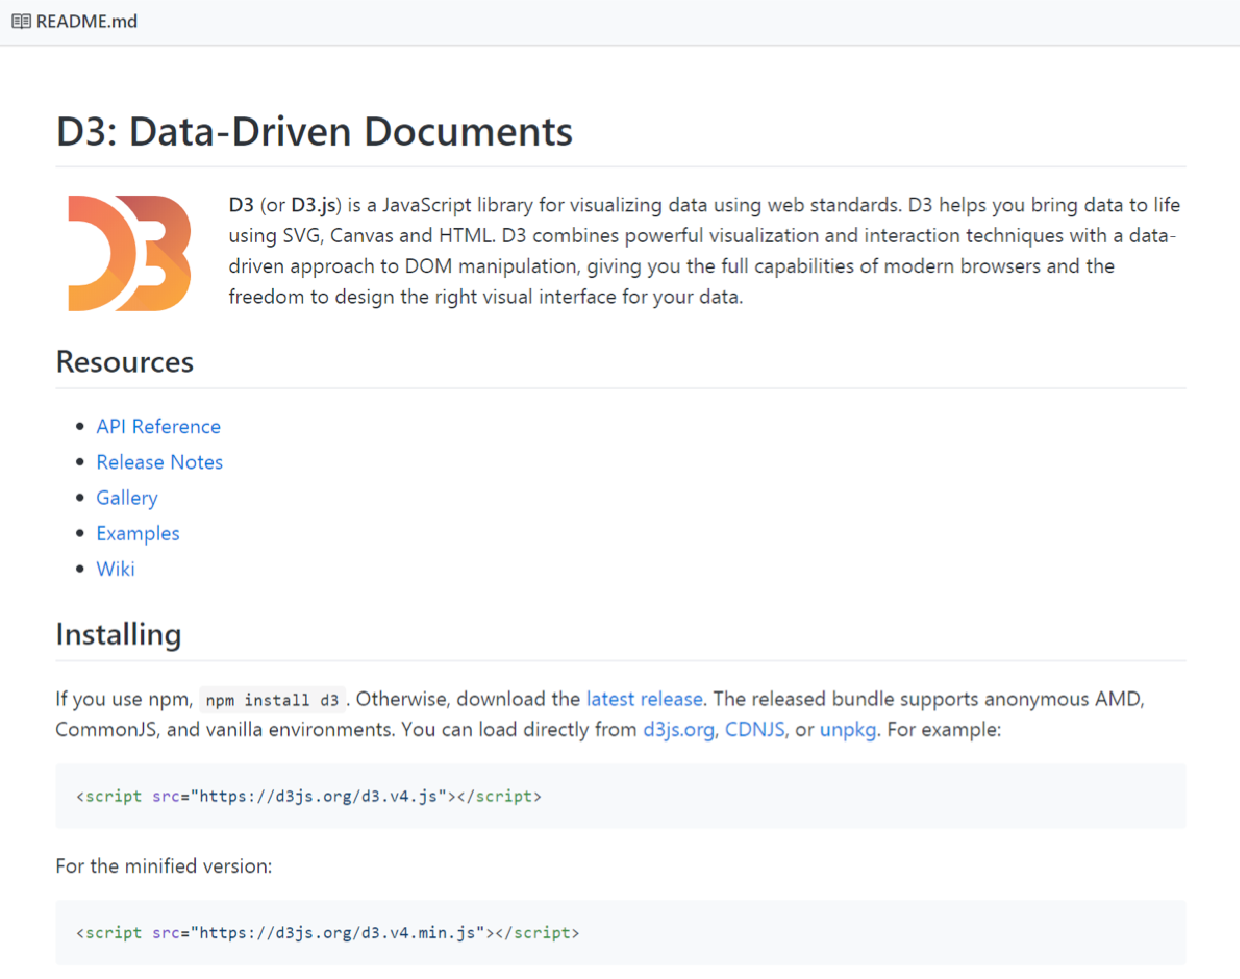
\includegraphics[width=1.0\linewidth]{./IPSJ202303_Ishioka/README_D3.pdf}
% 	\caption{READMEの例 JavaScriptライブラリ:D3}
%         \ecaption{hoge}
% 	\label{fig:oss_development}
% \end{figure}


%\textcolor{red}{henkoukasyo}

%% 2-2ーーーーーーーーーーーーーーーーーーーーーーーーーーーー
\subsection{関連研究}
\subsubsection{ソフトウェアドキュメントに関する研究}
ソフトウェアの情報を記述したドキュメントにはREADMEのほかに,APIドキュメントやリリースノートなどがある.

APIドキュメントには,ソフトウェアが提供するAPIのクラスやメソッド,細かな仕様などの情報が記述される.APIドキュメントを対象とした研究として,APIドキュメントの保守作業や作成支援のための研究が行われている.Maalejらは,JDK6と.NET4.0のプラットフォームにおけるAPIドキュメントの記述内容を調査している\cite{Ikeda_9_Maalej_API}.JDK6と.Net4.0から無作為に5,574件(JDK:2,792件,.NET:2,782件)抽出し,記述内容を調査した結果,APIドキュメントに記述される項目と項目ごとの記述傾向の違いを明らかにした.Zhouらは,APIドキュメントにおける欠陥の自動検出の手法を提案した\cite{APIDoc_Detection}.JDK1.8のAPIドキュメントを対象に手法の評価を行なった結果,適合率81.6\%,再現率82.0\%でAPIドキュメントの欠陥を検出することができた.

リリースノートは,ソフトウェアの更新履歴を記述したドキュメントで,ソフトウェアの前バージョンからの変更点や利用上の注意点などが記述される.リリースノートを対象とした研究として,記述内容の分析によって,開発者のリリースノート作成支援のための研究が行われている.Nathらは,コミットメッセージとマージプルリクエスト(PR)のタイトルからリリースノートを自動生成する手法を提案した\cite{RN_gen}.GitHubから取得した13のプロジェクトを対象にリリースノートを生成することで,提案手法の有用性を評価している.Abebeらは,85件のリリースノートの記述内容を調査した結果,記述すべきと考えられる項目を明らかにした.また,リリースノートに記載する項目を,機械学習を用いて推薦する手法を評価した結果,平均精度84\%,平均再現率90\%で,リリースノートに記載する項目を自動判別できた\cite{Ikeda_1_Abebe_note}.Morenoらは,990件のリリースノートを目視で確認することで,リリースノートに記述すべき項目を選定し,自動的に生成する手法を提案した\cite{Ikeda_11_Moreno_note}.また,53人の開発者を対象に提案手法を評価した結果,提案手法によって自動生成されたリリースノートは手動で作成されたリリースノートよりも優れており,正確であることを示した.

MaalejらはAPIドキュメント,AbebeらやMorenoらはリリースノート,本論文ではREADMEを対象としており,ソフトウェアドキュメントを分析するという点,ドキュメントの記述内容を分析する点で共通する.しかし,READMEはAPIドキュメントやリリースノートのように決まった形式で記述されず,開発者やプロジェクトによって記述方法が様々である点で異なる.

%% ーーーーーーーーーーーーーーーー
\subsubsection{READMEに関する研究}
開発者のREADME作成支援のための研究が行われている.

Pranaらは,READMEの作成支援を目的に,READMEの記述内容がいずれのカテゴリに属するのか,見出しを用いて自動分類し,ラベル付けする手法を提案した\cite{prana_README}.OSSから取得した393件のREADMEの各見出しを,著者が目視によって8つのカテゴリに分類し,分類の正しさを検証した.さらに評価実験を行った結果,提案手法(マルチラベル分類器)はF1値0.746を達成している.さらに,有用性の評価に参加したソフトウェア開発者の多くはPranaらの手法が有用であると回答している.READMEの見出しを項目に分類し,記述内容を分析している点で本論文と共通するが,本論文では最新版のREADMEだけでなく初期版からのREADMEを対象としている点,READMEの継時的変化を分析している点が異なる.Ikedaらは,開発者のREADME作成支援のために,READMEに記述される項目を分析した\cite{Ikeda_README}.GitHubから取得した43,911件のREADMEの各見出しを20項目に分類し,全体のプロジェクトに対する各項目の記述率について調査した.表2.1はIkedaらが分類した項目と記述率,分類された見出しの例を示す.調査の結果,対象プロジェクトの30%以上のREADMEに``Usage''(使用方法),``Install''(インストール方法),``License''(ライセンス)の項目が記述されていることが明らかとなった.READMEの見出しを項目に分類し,分析している点で共通するが,本論文では見出しだけでなく説明文の記述内容を対象としている点,最新版のREADMEだけでなく初期版からのREADMEを対象としている点,READMEの継時的変化を分析している点が異なる.亀井らは,開発者のドキュメント作成方法の推奨を目的に,REAMDEがどのように進化しているのか分析した\cite{Kamei_README}.GitHubから取得した365 件のプロジェクトを対象に,READMEの作成初期から最新版までの期間を4分割し,各期間でどのような項目が追加されたかを調査した.その結果,初期のREADMEにはプロジェクトの概要や利用方法に関する項目が記述され,プロジェクトの状態や貢献者に関する情報など開発者のための項目がREADMEに追加されることを明らかにした.また,READMEに記述される項目が増えるほど,プロジェクト全体の変更に対するREADME変更の割合が高くなることも明らかとなった.READMEの見出しを項目に分類し,READMEの項目の継時的変化に着目している点で共通するが,本論文では見出しだけでなく説明文の記述内容の継時的変化を対象としている点が異なる.



%\begin{table}[H]
% 	\centering
%	\caption{従来研究\cite{Ikeda_README}における記述項目一覧から引用}
%		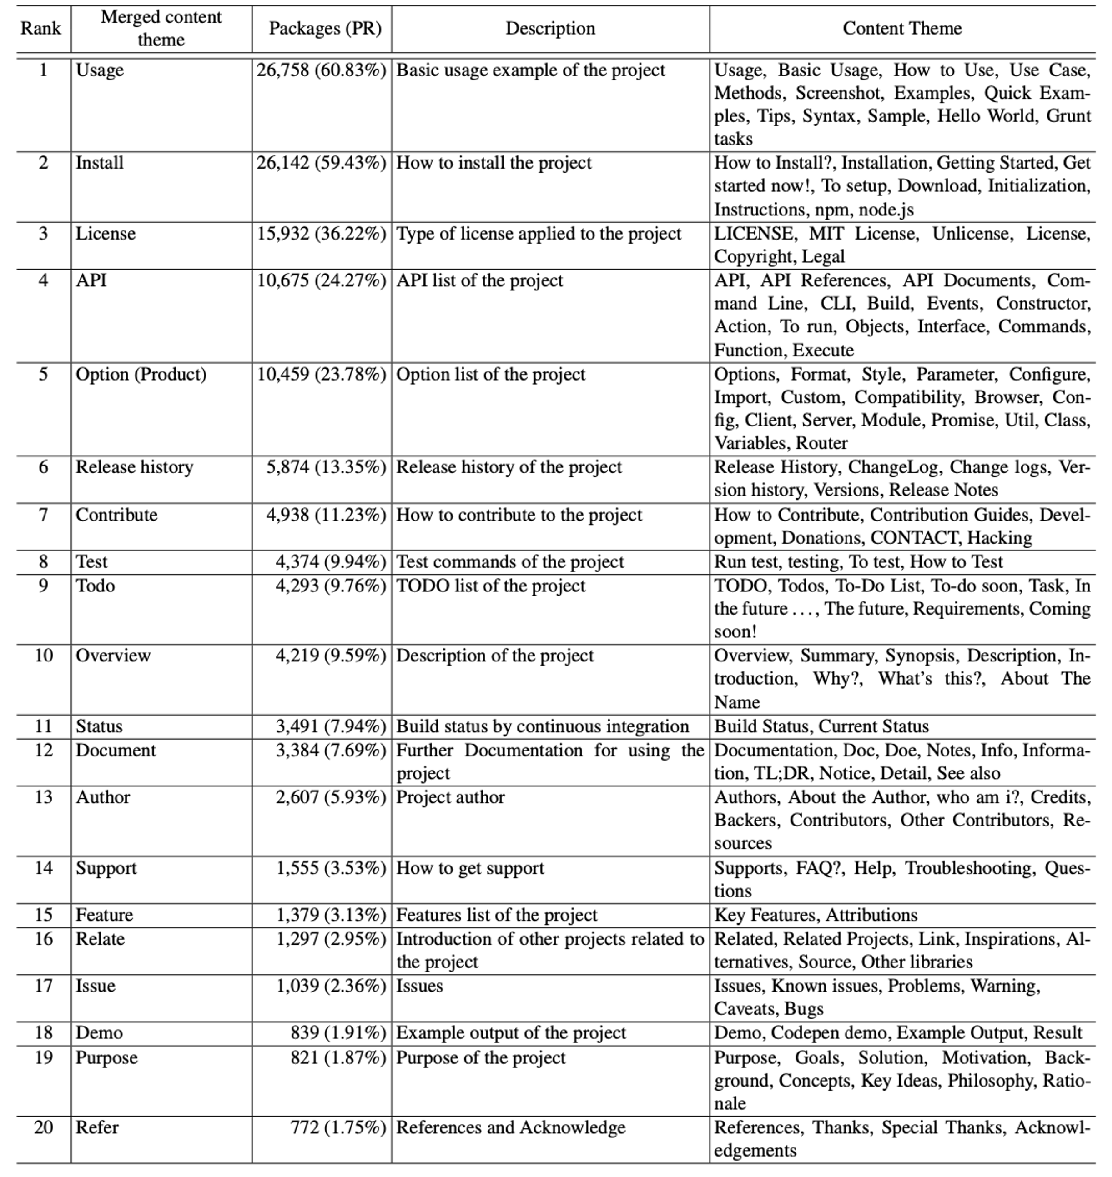
\includegraphics[width=1.0\linewidth]{./IPSJ202303_Ishioka/Ikeda_head_ieice.pdf}
%	\label{fig:oss_development}
%\end{table}

%    \textbf{正しい項目} & \textbf{項目「使用方法」と予測}\\
%    & \textbf{(16,590件)} \\ \hline \hline



% \begin{table*}[t]
% 	\centering
% 	\caption{従来研究\cite{Ikeda_README}における記述項目一覧から引用}
% 	\scalebox{0.7}{
% 	\begin{tabular}{r |l| l|l |l}
% 		\hline
% 		\textbf{Rank} & \textbf{Merged content} & \textbf{Packages(PR)} & \textbf{Description} & \textbf{Content Theme}\\
% 		 &\textbf{theme}&&\\
% 		\hline
% 		\hline
% 			\textbf{1} & Usage & 26,758(60.83\%) & Basic usage example of & Usage, Basic Usage, How to Use,  \\
% 			&&&the project&Use Case, Methods, Screenshot,  \\
% 			&&&&Examples, Quick Examples,Tips, Syntax, \\
% 			&&&&Sample, Hello World, Grunt tasks\\\hline
% 			\textbf{2} & Install & 26,142(59.43\%) & How to install the project & How to Install?, Installation, \\
% 			&&&& Getting Started, Get started now!, To setup, \\
% 			&&&&Download, Initialization, Instructions, \\
% 			&&&& npm, node.js\\\hline
% 			\textbf{3} & License & 15,932(36.22\%) & Type of license applied & LICENSE, MIT License, Unlicense, License,\\
% 			&&&to the project& Copyright, Legal\\\hline
% 			\textbf{4} & API & 10,675(24.27\%) & API list of the project & API, API References, API Documents,  \\
% 			&&&&Command Line, CLI, Build, Events, \\
% 			&&&&Constructor, Action, To run, Objects, \\
% 			&&&&  Interface, Commands, Function, Execute\\\hline
% 			\textbf{5} & Option & 10,459(23.78\%) & Option list of the project & Options, Format, Style, Parameter, \\
% 			&&&& Configure, Import, Custom, Compatibility, \\
% 			&&&&Browser, Config, Client,Server, Router,\\
% 			&&&& Module, Promise, Util, Class, Variables, \\\hline
			
% 			\textbf{6} & Release hitory & 5,874(13.35\%) & Release history of the project & Release History, ChangeLog,\\
% 			&&&& Change logs, Version history, Versions, \\
% 			&&&&Release Notes\\\hline
% 			\textbf{7} & Contribute & 4,938(11.23\%) & How to contribute to the  & How to Contribute, Contribution Guides, \\
% 			&&&project&Development, Donations, CONTACT, \\
% 			&&&&Hacking\\\hline
% 			\textbf{8} & Test & 4,374(9.94\%) & Test commands of the project & Run test, testing, To test, How to Test\\\hline
% 			\textbf{9} & ToDo & 4,293(9.76\%) & TODO list of the project & TODO, Todos, To-Do List, To-do soon, \\
% 			&&&&Task, In the future . . . , The future,\\
% 			&&&& Requirements, Coming soon!\\\hline
% 			\textbf{10} & Overview & 4,219(9.59\%) & Description of the project & Overview, Summary, Synopsis, \\
% 			&&&&Description, Introduction, Why?,\\
% 			&&&&  What’s this?, About The Name\\\hline
			
% 			\textbf{11} & Status & 3,491(7.94\%) & Build status by continuous & Build Status, Current Status\\
% 			&&&integration&\\\hline
% 			\textbf{12} & Document & 3,384(7.69\%) & Further Documentation for & Documentation, Doc, Doe, Notes, Info,\\
% 			&&&using the project&Information, TL;DR, Notice, Detail, See also\\\hline
% 			\textbf{13} & Author & 2,607(5.93\%) & Project author & Authors, About the Author, who am i?,  \\
% 			&&&&Credits, Backers, Contributors,\\
% 			&&&&Other Contributors, Resources\\\hline
% 			\textbf{14} & Support & 1,555(3.53\%) & How to get support & Supports, FAQ?, Help, Troubleshooting, \\
% 			&&&&Questions\\\hline
% 			\textbf{15} & Feature & 1,379(3.13\%) & Features list of the project & Key Features, Attributions\\\hline
			
% 			\textbf{16} & Relate & 1,297(2.95\%) & Introduction of other projects & Related, Related Projects, Link, Inspirations,\\
% 			&&&related to the project& Alternatives, Source, Other libraries\\\hline
% 			\textbf{17} & Issue & 1,039(2.36\%) & Issues & Issues, Known issues, Problems, Warning, \\
% 			&&&&Caveats, Bugs\\\hline
% 			\textbf{18} & Demo & 839(1.91\%) & Example output of the project & Demo, Codepen demo, Example Output, \\
% 			&&&&Result\\\hline
% 			\textbf{19} & Purpose & 821(1.87\%) & Purpose of the project & Purpose, Goals, Solution, Motivation, \\
% 			&&&&Background, Concepts, Key Ideas, \\
% 			&&&&Philosophy, Rationale\\\hline
% 			\textbf{20} & Refer & 772(1.75\%) & References and Acknowledge & References, Thanks, Special Thanks, \\
% 			&&&&Acknowledgements\\
% 		\hline
% 	\end{tabular}}
% 	\label{tab:file-comparison}
% \end{table*}





%% 2-3ーーーーーーーーーーーーーーーーーーーーーーーーーーーー
\subsection{本論文の位置付け}



従来研究\cite{prana_README}\cite{Ikeda_README}\cite{Kamei_README}では開発者のREADMEの作成支援を目的に,READMEに頻繁に記述される項目,また項目別に継時的変化を調査している.従来研究により,形式的なフォーマットが存在しないREADMEに記述する項目,またリポジトリ作成時に記述できない項目を明らかにすることは,新たにソフトウェアを公開する開発者にとって有用な知見である.しかし,READMEをどのように変更するのかは調査されておらず,開発者がソフトウェアの変更に伴いREADMEを変更しているのか否かも明らかにされていない.READMEはソフトウェアの進化に追従して変更されるべきドキュメントであるが,ソースコードを変更するたびにREADMEを変更するとは限らず,ファイルの変更に合わせて,開発者がREADMEを変更すべきか判断が困難であるため,開発者はREADMEの変更を見落とすと考えられる.開発者のREADME変更の作業負荷を低減させ,ソースコードの変更とともにREADMEが変更されるようにするためには,READMEの変更と直接関係があるファイルを把握する必要がある.

本論文では,開発者のREADME変更支援のために,同時に変更されるREADMEとその他ファイルの紐付け手法を提案する.本論文で提案するREADMEとその他のファイルの紐付け手法によって,READMEの変更とその他のファイルの変更を機械的に紐付けできれば,開発者のファイル変更に合わせて,README変更を開発者に推薦することで,開発者のREADME変更支援やREADMEを常に最新の状態にするといったREADMEの品質向上につながることを期待する.


%従来研究では開発者のREADMEの作成支援を目的に,READMEに頻繁に記述される項目,また項目の継時的変化を調査している.従来研究により,形式的なフォーマットが存在しないREADMEに記述する項目,またリポジトリ作成時に記述できない項目を明らかすることは,新たにソフトウェアを公開する開発者にとって有用な知見である.しかし,READMEをどのように変更するのかは調査されておらず,開発者がソフトウェアの変更に伴いREADMEを変更しているのか否かも明らかにされていない.READMEを常に最新の状態に保つために,開発者のREADME変更支援を行うには,READMEをどのように変更するのかを明らかにする必要がある.
%
%本論文では,開発者のREADME変更支援のために,READMEにおける各項目の変更方法,およびREADMEの変更と紐づくファイルを明らかにする2つの分析を行い,同時に変更されるREADMEとその他のファイルの紐付け手法を提案する.本論文成果によって,開発者のファイル変更に合わせたREADME変更の推薦を目指す.





%% 3章ーーーーーーーーーーーーーーーーーーーーーーーーーーーーーーーーーーーーーーーーーーーーーーーーーーー
\section{事前分析}
%% 3-1ーーーーーーーーーーーーーーーーーーーーーーーーーーーー
\subsection{データセット}
\subsubsection{対象プロジェクト}
本論文では,READMEにおける各項目の変更方法,およびREADMEの変更と紐づくファイルを明らかにする2つの分析において,大規模なソフトウェアエコシステムJavaScriptライブラリnpmで公開されるプロジェクトを対象として,次の手順で選定した.




\begin{enumerate}
  \item
  Witternら\cite{Ikeda_EN_9}と同様の手順で,2013年から2016年にGitHubにリポジトリを作成したプロジェクトをnpmから収集する.
%  \todo{これ本当?2016年までしか対象としないの?私のデータは2019年か2020年まであると思うけど...}
%→Yes:READMEの最新版が2016ではなく,この期間にnpmで作成されたJavaScriptプロジェクトの選定に用いているだけ.2020とかでない理由は,この手法は2016年にちょうど廃止されてしまったため.

  \item
  READMEの変更方法を分析するために,GitHubからクローンできたプロジェクトが作成したREADMEの開発履歴を収集する.
  
  \item
  リポジトリのトップページ以外に存在するREADMEは分析対象外とする.

  \item
  Markdown形式における見出し機能を利用していないREADMEは分析対象外とする.

  \item
  分析を容易にするため,英語以外の言語(日本語やハングル,キリル文字など)で記述されるREADMEは分析対象外とする.

  \item
  成熟したプロジェクトのREADMEを対象とするため,最終変更から1年以上経過しているREADMEを対象とする.
  
\end{enumerate}

最終的に,52,292件のプロジェクトのREADMEを分析対象とする.


\subsubsection{READMEからの項目と説明文の抽出}
READMEには本文を要約した見出しが文章の前に記述される.開発者はMarkdown形式で「\#」と共に見出しを記述する.本論文では,\#1つ(h1:大見出し)および\#2つ(h2:中見出し)を見出しとして抽出する.また本論文では,Ikedaら\cite{Ikeda_README}が分類した20項目を使用し,抽出した見出しを分類する.次に,見出しから次の見出しまでに記述される文章を説明文として抽出する.最終的に,167,782件の項目と説明文のペアをデータセットとする.



%% 3-2ーーーーーーーーーーーーーーーーーーーーーーーーーーーー
\subsection{事前分析の概要}
READMEの変更には,ソースコードの変更とともにREADMEを変更する場合と,READMEのリファクタリングを行う場合の2種類が考えられる.この内,READMEのリファクタリングを目的とした変更は,ソースコードの変更とは無関係で,本論文で提案する,READMEの変更とその他のファイルの変更の紐付け手法の性能を低下させる要因になると考える.事前分析では,このようなソースコードの変更とは無関係なREADMEの変更が行われる可能性のある項目を確認する.


従来研究\cite{Ikeda_README}は,READMEの見出しを20項目に分類し,多くのプロジェクトで共通して記述する項目を明らかにしているが,各項目と説明文の内容が一致しているか否かは定量的に明らかにしていない.そこで,各項目と説明文の内容が一致している(項目と説明文に一貫性がある)場合,開発者はソースコードの変更とともに,その変更内容に関する記述を,READMEの項目ごとに変更(追加,削除)すると考える.一方で,各項目と説明文の内容が一致しない(項目と説明文に一貫性がない)場合は,READMEのリファクタリングを目的に,ソースコードの変更とは無関係に,説明文を異なる項目へ移動する修正を加えると考える.ソースコードの変更とは独立したREADME単体での変更が頻繁に行われる場合,ソースコードの変更との依存関係を考慮できないため,その変更意図や目的を正確に理解することが困難になる.各項目と説明文の内容が一致しているか否かを明らかにするために,事前分析ではREADMEの各項目に対する説明文の一貫性を調査する.具体的には,3.1節で抽出したプロジェクトのREADMEを対象に,READMEの説明文から20項目を分類するための多クラス分類モデルを構築することで,各項目の説明文がプロジェクト間で共通しているのかを明らかにする.



%従来研究\cite{Ikeda_README}は,READMEの見出しを20項目に分類し,多くのプロジェクトで共通して記述する項目を明らかにしているが,各項目の説明文には同一の内容が記述されているか否かは定量的に明らかにしていない.各項目の説明文に同一の内容が記述される(項目と説明文に一貫性がある)場合,開発者はREADMEの項目単位で個別に修正(追加,削除)することが示唆される.一方で,同一の内容が異なる項目に記述されている(項目と説明文に一貫性がない)場合,開発者は説明文を異なる項目へ移動する修正を加えることも示唆される.説明文をREADMEの中で移動する場合,README単体で修正されるため,ソースコードの変更とソフトウェアの変更に伴う変更に限らないことがわかる.ソースコードの変更とは独立したREADME単体での変更が頻繁に行われる場合,ソースコードの変更やソフトウェアの変更との依存関係を考慮できないため,その変更意図や目的を正確に理解することが困難になる.各項目の説明文に同一の内容が記述されているか否かを明らかにするために,事前分析ではREADMEの各項目に対する説明文の一貫性を調査する.具体的には,3.1節で抽出したプロジェクトのREADMEを対象に,READMEの説明文から20項目を分類するための多クラス分類モデルを構築することで,各項目の説明文がプロジェクト間で共通しているのかを明らかにする.




%% 3-3ーーーーーーーーーーーーーーーーーーーーーーーーーーーー
\subsection{事前分析の手法}

%% 3-3-1ーーーーーーーーーーー
\subsubsection{分析手順}
同じ内容が異なる項目の説明文に記述されているか否か,項目と説明文の一貫性を確認するために,READMEの説明文から20項目を分類する多クラス分類モデルを構築する.READMEの説明文を分類モデルの説明変数として使用するために,説明文に対して,記号などの削除,分かち書き,ストップワードの除去,表記の統一,ベクトル化の順でデータを整形する.目的変数はREADMEに記述される見出しを分類した20項目を使用する.分類結果の評価は,再現率と適合率を用いて評価する.

%% 3-3-2ーーーーーーーーーーー
\subsubsection{説明変数のデータ整形}
本節では,READMEの説明文に記述される単語を説明変数として使用し,分類モデルに入力するための前処理を行う.

\begin{enumerate}
  \item{\textbf{記号などの除去:}}
  READMEはMarkdown形式で記述されるため,プログラムや記号などが含まれる.本論文では,自然言語で記述される単語を対象とするため,説明文に含まれるURLの削除,プログラムや記号の除去を正規表現を用いて行う.
  \item{\textbf{形態素解析:}}
  説明文を単語ごとに分解し,各単語の品詞を判別する.文章から,品詞ごとに分けてそれぞれを1つの単語とする.
  \item{\textbf{ストップワード除去:}}  
  Pythonのnltk.corpus.stopwordsに含まれる単語(前置詞や接続詞,代名詞,冠詞,助動詞)を除去する.
  \item{\textbf{レンマ化:}}
  形態素解析で判明した品詞をもとに,語幹の統一を行う.現在進行形や複数形,過去形の単語を標準形に統一することである.この処理には,Pythonのnltk.stem.wordnetのlemmatizeモジュールを利用して語幹の統一を行う.また,単語の大文字は全て小文字表記に統一する.
  \item{\textbf{ベクトル化(Bag of Words):}}
  予測モデル構築において,READMEの説明文に記述される単語を説明変数として扱うためにベクトル化を行う.ベクトル化には,PythonモジュールであるgensimのBag of Words~\footnote[5]{https://www.tutorialspoint.com/gensim/gensim\_creating\_a\_bag\_of\_words\_corpus.html}を使用する.Bag of Wordsは自然言語で記述された文書に含まれる単語を出現回数に基づきベクトル化する手法である.
\end{enumerate}

%% 3-3-3ーーーーーーーーーーー
\subsubsection{READMEの項目を分類するモデルの構築}
分類モデル構築のために,READMEの20項目を目的変数として計測する.3.3.2でデータ整形を行ったREADMEの説明文を説明変数とし,READMEの項目に分類するモデルを構築する.データセットの8割を学習用データとしてモデルを構築し,残り2割をテスト用データとする.

本論文では,分類モデルの構築に機械学習アルゴリズムであるランダムフォレスト\cite{random_forest}を用いる.ランダムフォレストは,学習データから複数の決定木を作成するアンサンブル学習法である.ランダムフォレストの利点としては,学習データの標準化を必要としない点,過学習を防ぎ汎化性能が高い点,予測精度に説明変数がどの程度寄与したかを示す特徴量の重要度を算出できる点などが挙げられる.ランダムフォレストの実装には,Pythonのsklearn.ensemble.RandomForestClassifier~\footnote[6]{https://scikit-learn.org/stable/modules/generated/sklearn.ensemble.RandomForestClassifier.html}を用いる.ランダムフォレストの木の数はデフォルト値である100,各決定木作成に使用する説明変数の数はすべての説明変数の数の平方根を使用する.


%% 3-3-4ーーーーーーーーーーー
\subsubsection{評価方法}
% モデルの分類結果から,項目の分類結果と実際の項目を合わせた表3.1の混同行列を作成する.表3.1はTP,FP,TN,FNの4つで構成される.

% %-----------------------
% \begin{table}[t]
%  \centering
%  \caption{モデルの分類結果と正解の比較}
%  \ecaption{hoge}
% \label{tab:result}
%   \scalebox{1.0}{
%   \begin{tabular}{c|c|c} \hline
%      & \textbf{正しい項目と予測} & \textbf{別の項目と予測} \\ \hline
%     \textbf{正しい項目} & TP & FN \\ \hline
%     \textbf{別の項目} & FP & TN \\ \hline
%   \end{tabular}
%     \label{tab:result}
%    }
% \end{table}
% %-----------------------


% \begin{itemize}
%   \item TP (True Positive) : 対象の項目を,正しい項目に分類
%   \item FP (False Positive) : 別の項目を,対象の項目であると誤って分類
%   \item TN (True Negative) : 別の項目を,別の項目であると正しく分類
%   \item FN (False Negative) : 対象の項目を,別の項目であると誤って分類
% \end{itemize}


評価指標には,一般的に機械学習モデルの評価に用いられる適合率,再現率,F1値を用いる.
% それぞれの評価指標を以下に示す.

% 適合率とは,項目を分類した結果が,対象の項目であった割合を示す.
% \begin{equation}
% \label{calculate_Precision}
%  適合率 = \frac{TP}{TP + FP}
% \end{equation}

% 再現率とは,対象の項目のうち,分類モデルによって正しく分類された割合を示す.
% \begin{equation}
% \label{calculate_Recall}
% 再現率 = \frac{TP}{TP + FN}
% \end{equation}

% 適合率と再現率はトレードオフの関係であるため,再現率と適合率の調和平均であり,総合的な評価の際に利用されるF1値でも評価を行う.F1値は0から1の間の値で示され,値が高いほどモデルの評価も高くなる.
% \begin{equation}
% \label{calculate_F}
%  F値 = \frac{2 * 再現率 * 適合率}{再現率 + 適合率}
% \end{equation}

% 以上の評価指標を基に,適合率と再現率の解釈について述べる.




%\begin{itemize}
%  \item 適合率,再現率ともに高い項目: 特定の内容が特定の項目に記述され,項目と説明文に一貫性がある
%  \item 適合率が高く,再現率が低い項目 : 項目と説明文に一貫性はあるが,多様な内容が特定の項目に記述される
%  \item 再現率が高く,適合率が低い項目 : 特定の内容が異なる項目にも記述され,項目と説明文に一貫性がない
%\end{itemize}

%\begin{itemize}
%  \item 適合率,再現率ともに高い項目: 説明文がプロジェクト間で共通しており,項目と説明文に一貫性がある.
%  \item 適合率が高く,再現率が低い項目 : 項目と説明文に一貫性はあるが,多様な内容が特定の項目に記述され,説明文がプロジェクト間で共通しない
%  \item 適合率が低く,再現率が高い項目 : 説明文がプロジェクト間で共通するが,特定の内容が異なる項目にも記述され,項目と説明文に一貫性がない
%\end{itemize}

%P↑ → 項目Aに記述される固有の内容はあるが,それが複数ある. →一貫性はある(各項目の内容が記述される,種類がたくさんなだけ)
%R↑ → 項目Aに記述される内容が,他の項目に登場する.→一貫性はある(各項目の内容が記述される,他にも出てくるだけ)

%\begin{itemize}
%  \item 適合率,再現率ともに高い項目: 説明文がプロジェクト間で共通しており,項目と説明文に一貫性がある.
%  \item 適合率が高く,再現率が低い項目 : 項目と説明文に一貫性はあるが,多様な内容が特定の項目に記述される.
%  \item 適合率が低く,再現率が高い項目 : 項目と説明文に一貫性はあるが,特定の内容が異なる項目にも記述される.
%\end{itemize}

%\begin{itemize}
%  \item 適合率,再現率ともに高い項目: 説明文がプロジェクト間で共通しており,項目と説明文に一貫性がある.
%  \item 適合率が高く,再現率が低い項目 : \textcolor{red}{項目と説明文に一貫性はあるが,多様な内容が項目に記述されるため,説明文がプロジェクト間で共通しない.}
%  \item 適合率が低く,再現率が高い項目 : \textcolor{red}{説明文がプロジェクト間で共通しているが,項目の内容が異なる項目にも記述されており,ソースコードの変更と無関係なREADME単体での変更が行われる可能性がある..}
%\end{itemize}


\begin{itemize}
  \item 適合率: 適合率は,項目を分類した結果が,対象の項目であった割合を示す.適合率が高い場合,項目と説明文に一貫性があり,ソースコードの変更とともに,項目ごとに説明文を変更する.適合率が低い場合,項目の内容が異なる項目にも記述されており,ソースコードの変更と無関係なREADME単体での変更が行われる可能性がある
  \item 再現率: 対象の項目のうち,分類モデルによって正しく分類された割合を示す.再現率が高い場合,説明文がプロジェクト間で共通している.再現率が低い場合,プロジェクトの特性によって異なり,多様な内容が項目に記述されるため,一般的な結論を導くことが難しい.
\end{itemize}





%% 3-4ーーーーーーーーーーーーーーーーーーーーーーーーーーーー
\subsection{事前分析の結果}
図3.1はモデルが分類した各項目の適合率と再現率を表す.横軸は適合率,縦軸は再現率を表し,各点がそれぞれの項目を表す.また,表3.2は各項目の適合率,再現率,F1値,データ数を示す.結果から,項目「ライセンス(適合率=0.89,再現率=0.99,F1値=0.94)」や「貢献方法(適合率=0.89,再現率=0.88,F1値=0.89)」,「テスト(適合率=0.87,再現率=0.76,F1値=0.81)」は他の項目と比べ,適合率,再現率,F1値が高く,これらの項目の説明文はプロジェクト間で共通しており,項目と説明文に一貫性があることが示唆される.

また,項目「使用方法」を除く多くの項目は適合率が高く,項目と説明文に一貫性があり,ソースコードの変更とともに,項目ごとに説明文を変更することが考えられる.

適合率が低く再現率が高い項目「使用方法」の説明文に記述された内容は,他の項目の説明文にも記述されていると考えられる.表3.3は,図3.1および表3.2において,どの項目と誤分類したかを示す.分析の結果,API(1,671件)や概要(1,007件),オプション(976件)などの項目は,項目「使用方法」であると誤分類されており,項目「使用方法」の説明文には類似する内容(例:使用するAPIの説明,オプションの設定方法など)が記述されていると考えられる.項目「使用方法」では,異なる項目(API,概要,オプション)への説明文の内容の移動を行うことが考えられる.


事前分析の結果から,項目「ライセンス」や「貢献方法」などの多くの項目は,項目と説明文に一貫性があり,開発者はソースコードの変更とともに,項目ごとに説明文の内容の追加や削除を行うと考えられる.項目「使用方法」の説明文に記述された内容は,他の項目の説明文にも記述されている可能性があるため,項目「使用方法」は,説明文の内容の追加や削除だけでなく,異なる項目への説明文の内容の移動を行うことが考えられる.異なる項目への説明文の移動を行うのであれば,READMEはソースコードの変更に伴う変更だけでなく,README単体で変更を行う可能性がある.ソースコードの変更とは独立したREADME単体での変更が頻繁に行われる場合,ソースコードの変更との依存関係を考慮できないため,その変更意図や目的を正確に理解することが困難になる.また,本論文で提案する,READMEの変更とその他のファイルの変更の紐付け手法の性能を低下させる要因になると考える.分析1では,このようなソースコードの変更とは無関係なREADMEの変更が行われているか,また,項目ごとに説明文の内容の追加や削除が行われているのかを明らかにする.分析2では,本論文で提案するREADMEとその他のファイルの紐付け手法によって,READMEの変更とその他のファイルの変更を機械的に紐付けることができるのかを明らかにする.



%分析1では,READMEの項目単位での変更(追加,削除)や異なる項目への説明文の移動が行われているのかを明らかにする.分析2では,README変更がソースコードの変更と紐づいているのか,機械的にREADME変更とソースコードの変更を紐付けることができるのかを明らかにする.





%-----------------------
\begin{figure}[t]
 	\centering
		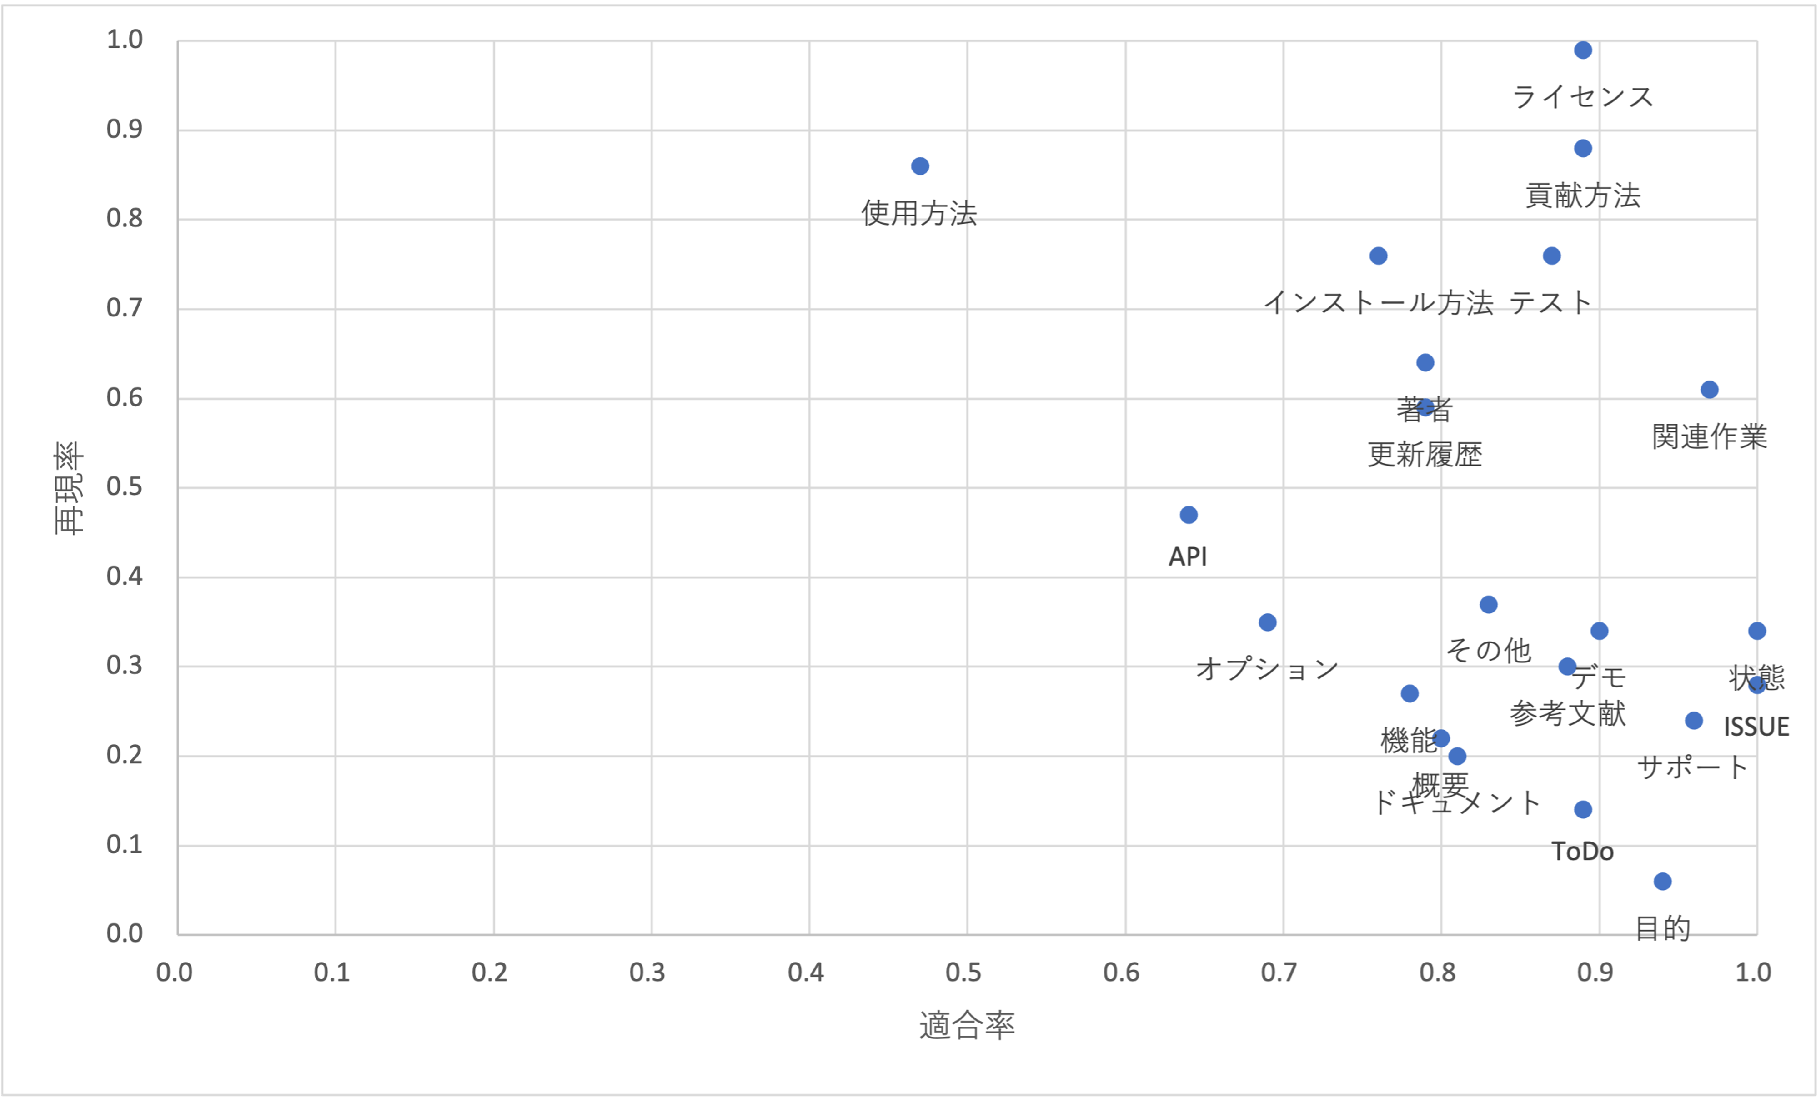
\includegraphics[width=1.0\linewidth]{./IPSJ202303_Ishioka/maluti_PR.pdf}
	\caption{事前分析の結果}
	\label{fig:oss_development}
\end{figure}
%-----------------------


%---------------------------------------------------------

%-----------------------
\begin{table}[t]
\centering
\caption{20項目の分類結果}
\label{tab:data}
\begin{tabular}{l|r|r|r|r}
\hline\hline
項目 & 適合率 & 再現率 & F1値 & データ数 \\
\hline
使用方法 & 0.47 & 0.86 & 0.86 & 9,003 \\\hline
インストール方法 & 0.76 & 0.76 & 0.76 & 4,196 \\\hline
ライセンス & 0.89 & 0.99 & 0.94 & 2,420 \\\hline
API & 0.64 & 0.47 & 0.54 & 3,615 \\\hline
オプション & 0.69 & 0.35 & 0.47 & 1,771 \\\hline
更新履歴 & 0.79 & 0.59 & 0.68 & 722 \\\hline
貢献方法 & 0.89 & 0.88 & 0.89 & 2,093 \\\hline
テスト & 0.87 & 0.76 & 0.81 & 493 \\\hline
ToDo & 0.89 & 0.14 & 0.25 & 487 \\\hline
概要 & 0.80 & 0.22 & 0.34 & 1,476 \\\hline
状態 & 1.00 & 0.34 & 0.51 & 62 \\\hline
ドキュメント & 0.81 & 0.20 & 0.33 & 593 \\\hline
著者 & 0.79 & 0.64 & 0.71 & 318 \\\hline
サポート & 0.96 & 0.24 & 0.39 & 193 \\\hline
機能 & 0.78 & 0.27 & 0.40 & 941 \\\hline
関連 & 0.97 & 0.61 & 0.75 & 189 \\\hline
Issue & 1.00 & 0.28 & 0.43 & 112 \\\hline
デモ & 0.90 & 0.34 & 0.50 & 76 \\\hline
目的 & 0.94 & 0.06 & 0.12 & 265 \\\hline
リファレンス & 0.88 & 0.30 & 0.45 & 201 \\
\hline
\end{tabular}
\end{table}
%-----------------------


%---------------------------------------------------------




%-----------------------
\begin{table}[t]
 \centering
 \caption{項目「使用方法」の予測結果}
\label{tab:result}
  \scalebox{1.0}{
  \begin{tabular}{l|r} 
  \hline\hline
    正しい項目 & 項目「使用方法」と予測\\
    & (16,590件) \\ \hline
    使用方法 & 7,723件(47\%)\\ \hline
    その他 & 1,954件(12\%)\\ \hline
    API & 1,671件(10\%)\\ \hline
    概要 & 1,007件(6\%)\\ \hline
    オプション & 976件(6\%)\\ \hline
    インストール方法 & 937件(6\%)\\ \hline
    機能の説明 & 594件(4\%)\\ \hline
      : & : \\ 
  \hline
  \end{tabular}
    \label{tab:result}
   }
\end{table}
%-----------------------




%% 4章ーーーーーーーーーーーーーーーーーーーーーーーーーーーーーーーーーーーーーーーーーーーーーーーーーーー
\section{分析1: READMEの項目はどのように変更されるのか?}
%% 4-1ーーーーーーーーーーーーーーーーーーーーーーーーーーーー
\subsubsection{概要}
%3章の事前分析の結果から,項目「使用方法」以外の項目は,プロジェクト間で項目と説明文に一貫性があり,開発者はREADME変更時,項目ごとに説明文の内容の追加や削除を行うと考えられる.また,項目「使用方法」では,異なる項目への説明文の移動が行われる可能性がある.本章では,READMEの同一項目での変更 (追加,削除) や異なる項目への説明文の移動が行われているのかを明らかにする.具体的には,初期版と最終版のREADMEに記述される項目および説明文を比較し,READMEの変更において,各項目の説明文がどのように変更されるのかを分類する.READMEの変更方法には,同じ項目の説明文が変更される場合と異なる項目へ跨って説明文が変更される場合の2通り考えられる.
3章の事前分析の結果から,項目「使用方法」以外の項目は,項目と説明文に一貫性があり,開発者はソースコードの変更とともに,項目ごとに説明文の内容の追加や削除を行うと考えられる.また,項目「使用方法」では,説明文の内容の追加や削除だけでなく,異なる項目への説明文の移動が行われる可能性がある.本章では,READMEの同一項目での変更 (追加,削除) や異なる項目への説明文の移動が行われているのかを明らかにする.具体的には,初期版と最終版のREADMEに記述される項目および説明文を比較し,READMEの変更において,各項目の説明文がどのように変更されるのかを分類する.READMEの変更方法には,同じ項目の説明文が変更される場合と異なる項目へ跨って説明文が変更される場合の2通り考えられる.


\subsubsubsection{同じ項目の説明文が変更される場合}
ソースコードの変更とともに,説明文の内容の追加や削除を行うと考えられる.
\begin{itemize}
  \item 追加 : 既存の説明文に新しい情報を説明文に追加
  \item 削除 : 不要な情報を説明文から削除
\end{itemize}

\subsubsubsection{異なる項目へ説明文が移動される場合}
異なる項目へ跨った変更は説明文の記述内容が類似する項目間で起こると考えられる.ソースコードの変更とは無関係な,READMEのリファクタリングを行うと考えられる.
\begin{itemize}
  \item 細分化 : 1つの項目の内容を,複数の項目に分割して移動
  \item 統合 : 複数の項目の内容を,1つの項目に統合して移動
\end{itemize}


追加,削除,細分化,統合を明確に分類することで,READMEの同一項目での変更 (追加,削除) や異なる項目への説明文の移動が行われているのかを明らかにする.



%% 4-2ーーーーーーーーーーーーーーーーーーーーーーーーーーーー
\subsection{データセット}
3章の事前分析同様に,52,292件のプロジェクトのREADMEを分析対象とし,READMEから項目と説明文を抽出する.本章では,READMEの変更を分析するために,初期版と最終版のREADMEに記述される項目および説明文を抽出し,データセットとして使用する.




%% 4-3ーーーーーーーーーーーーーーーーーーーーーーーーーーーー
\subsection{手法}
初期版と最終版のREADMEの項目数および各項目に記述される説明文を比較し,READMEの変更方法(追加,削除,細分化,統合)を分類する.具体的には,初期版と最終版のREADMEの説明文の一致率,連続一致率,文字数を比較する.同一項目間と異なる項目間で説明文の比較方法が異なるため,それぞれの分析手法を順に記述する.


%% ーーーーーーーーーーーーーーーー
\subsubsection{同じ項目の説明文が変更される場合}
初期版と最終版READMEにおける同一項目間で説明文を比較する.比較方法には,文章の一致率を用いる.文章の一致率とは,同一項目間でどれだけ説明文が共通するかを表す指標である.一致率が高く,文字数が初期版から最終版READMEにかけて増加している場合は,READMEの変更「追加」が行われている.一致率が高く,文字数が初期版から最終版READMEにかけて減少している場合は,READMEの変更「削除」が行われていると判断する.

%

\begin{equation}
\label{calculate_rate}
\mbox{一致率} = \frac {\mbox{最長共通部分列}} {\mbox{初期版READMEの文字数}}
\end{equation}
\vspace{5pt}



最長共通部分列(Longest Common Subsequence)は,初期版と最終版READMEの同一項目における説明文で共通する文字列の最大値(文字列は不連続でも出現する順序のみを考慮)のことである.図4.1は,項目「使用方法」の初期版から最終版で追加された箇所が,連続する場合と不連続する場合の例を示す.左の例では,初期版に存在した110文字を元に,後ろに文章を追加した例で,元の内容が100\%含まれているため,最長共通部分列は110,この時の一致率は110/110(100\%)となる.この例では,一致率が100\%と高く,文章量が初期版と比べ増加しているため,READMEの変更「追加」が行われていると判断する.右の例では,初期版に存在した110文字の間に文章が追加され,元の文章が連続しないが,元の内容が100\%含まれていることを,最長共通部分列の値から確認できる.情報の追加,削除箇所に関わらず,同一項目間の変更(追加,削除)を捉えることができるため,同一項目間での比較の際には最長共通部分列を使用する.


%--------------------------------
\begin{figure}[t]
 	\centering
		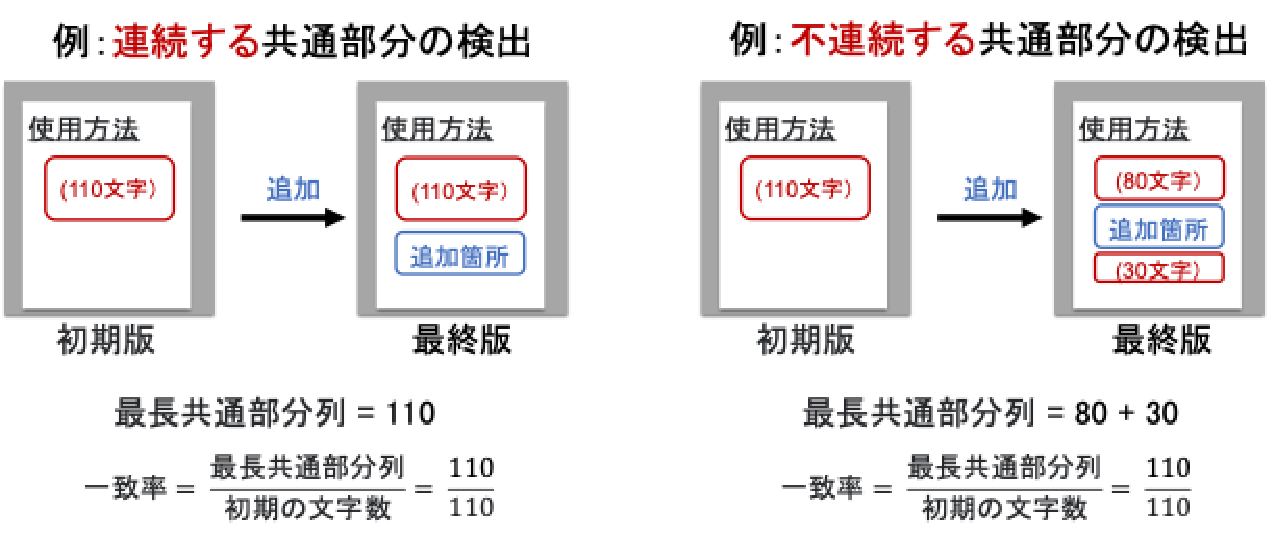
\includegraphics[width=1.0\linewidth]{./IPSJ202303_Ishioka/LCS_add.pdf}
	\caption{同じ項目での比較例}
	\label{fig:oss_developments_eq}
\end{figure}
%--------------------------------






%% ーーーーーーーーーーーーーーーー
\subsubsection{異なる項目へ説明文が移動される場合}
初期版と最終版READMEにおける異なる項目間で説明文を比較する.比較方法には,文章の連続一致率を用いる.文章の連続一致率とは,異なる項目間で初期版の説明文の内容がどれだけ存在するかを表す指標である.連続一致率が高い場合は,READMEの変更「細分化,統合」が行われている可能性がある.連続一致率が低い場合は,READMEの変更「細分化,統合」は行われていないと判断する.

\begin{equation}
\label{calculate_rate}
\mbox{連続一致率} = \frac {\mbox{最長共通部分文字列}} {\mbox{初期版READMEの文字数}}
\end{equation}
\vspace{5pt}

ここで用いられる最長共通部分文字列(Longest Common Substrings)とは,初期版と最終版READMEの異なる項目における説明文で連続して共通する文字列の最大値のことである.図4.2は,異なる項目への移動が行われていない場合の例を示す.この例だと,初期版の項目「使用方法」に存在した110文字が,最終版の項目「オプション」の説明文内に5文字一致,3文字一致,など合計して90文字共通する文字が存在し,最大で共通する文字列の長さが5文字であることを表す.ここで,同じ項目での比較時同様に最長共通部分列を用いた場合,一致率は90/110(82\%)となってしまい,情報の移動の可能性があると誤検出してしまう.一方で,最大共通部分文字列を用いた場合,連続一致率が5/110(5\%)となり,関係がないと判断できる.誤検出を防ぐことができるため,異なる項目間での比較の際には最長共通部分文字列を使用する.

%--------------------------------
\begin{figure}[t]
 	\centering
		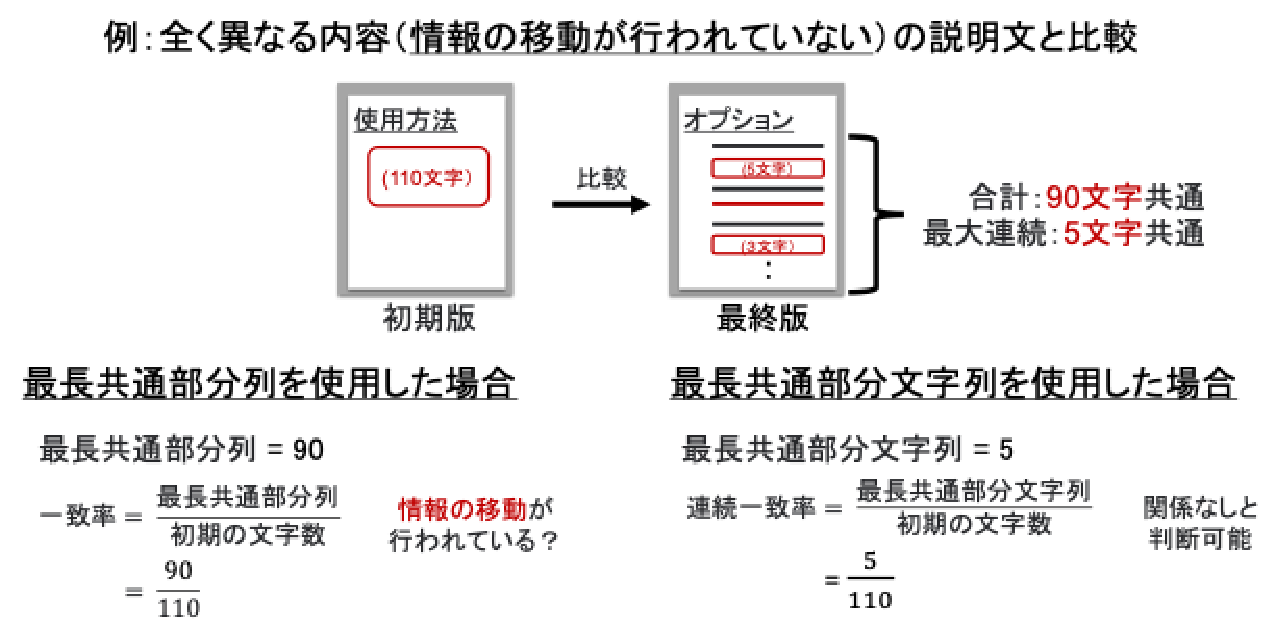
\includegraphics[width=1.0\linewidth]{./IPSJ202303_Ishioka/LCS_split.pdf}
	\caption{異なる項目での比較例}
	\label{fig:oss_developments_eq}
\end{figure}
%--------------------------------


%% 4-4ーーーーーーーーーーーーーーーーーーーーーーーーーーーー
\subsection{結果}
表4.1は初期版と最終版READMEの項目数の平均,中央値を示す.表4.2は初期版から最終版READMEにかけて追加,削除された項目数の平均,中央値,項目数が変化したリポジトリ数を示す.結果から,多くのリポジトリにおいて項目の追加が行われていた.

%--------------------------------
\begin{table}[t]
 \centering
 \caption{初期版と最終版READMEの項目数}
\label{tab:result}
  \scalebox{1.0}{
  \begin{tabular}{l|r|r} \hline
     & 平均値 & 中央値\\ \hline
    初期版項目数 & 2.63 & 2.00\\ \hline
    最終版項目数 & 4.06 & 4.00 \\ \hline
    追加項目数 & 2.92 & 2.00 \\ \hline
    削除項目数 & 2.24 & 2.00 \\ \hline
  \end{tabular}
     }
\end{table}
%--------------------------------
\begin{table}[t]
 \centering
 \caption{初期版と最終版READMEの項目数の変化}
\label{tab:result}
  \scalebox{1.0}{
    \begin{tabular}{l|r} \hline
     & リポジトリ数\\ \hline
    項目を追加 & 27,045\\ \hline
    変更なし & 18,327\\ \hline
    項目を削除 & 3,895\\ \hline
    合計 & 49,267\\ \hline
  \end{tabular}
    \label{tab:result}
   }
\end{table}

%--------------------------------

\subsubsection{同じ項目での比較}
図4.3は初期版と最終版READMEの説明文を同じ項目同士で比較した一致率の分布を示す.横軸は一致率を表し,縦軸は項目数を表す.一致率が高いほど,READMEの変更「追加」や「削除」が行われる可能性が高いことを示す.赤は初期版と最終版READMEの同一項目における説明文の一致率が高く,文字数が増加している変更「追加」,緑は初期版と最終版READMEの同一項目における説明文の一致率が高く,文字数が変化していない「変更なし」,青は初期版と最終版READMEの同一項目における説明文の一致率が高く,文字数が減少している変更「削除」を表す.結果から,同一項目において,初期版と最終版READMEの説明文は一致率が高く,初期版の説明文の内容を基に変更されていた.また,一致率が高い(90-100\%)説明文を確認したところ,69,986件のうち「追加」が行われたのが32,070件,「変更なし」が33,871件,「削除」が行われたのが4,045件であった.図4.3の結果から,README変更において「削除」が行われることは少なく,「追加」が行われることが多いことを確認した.

%--------------------------------
\begin{figure}[t]
 	\centering
		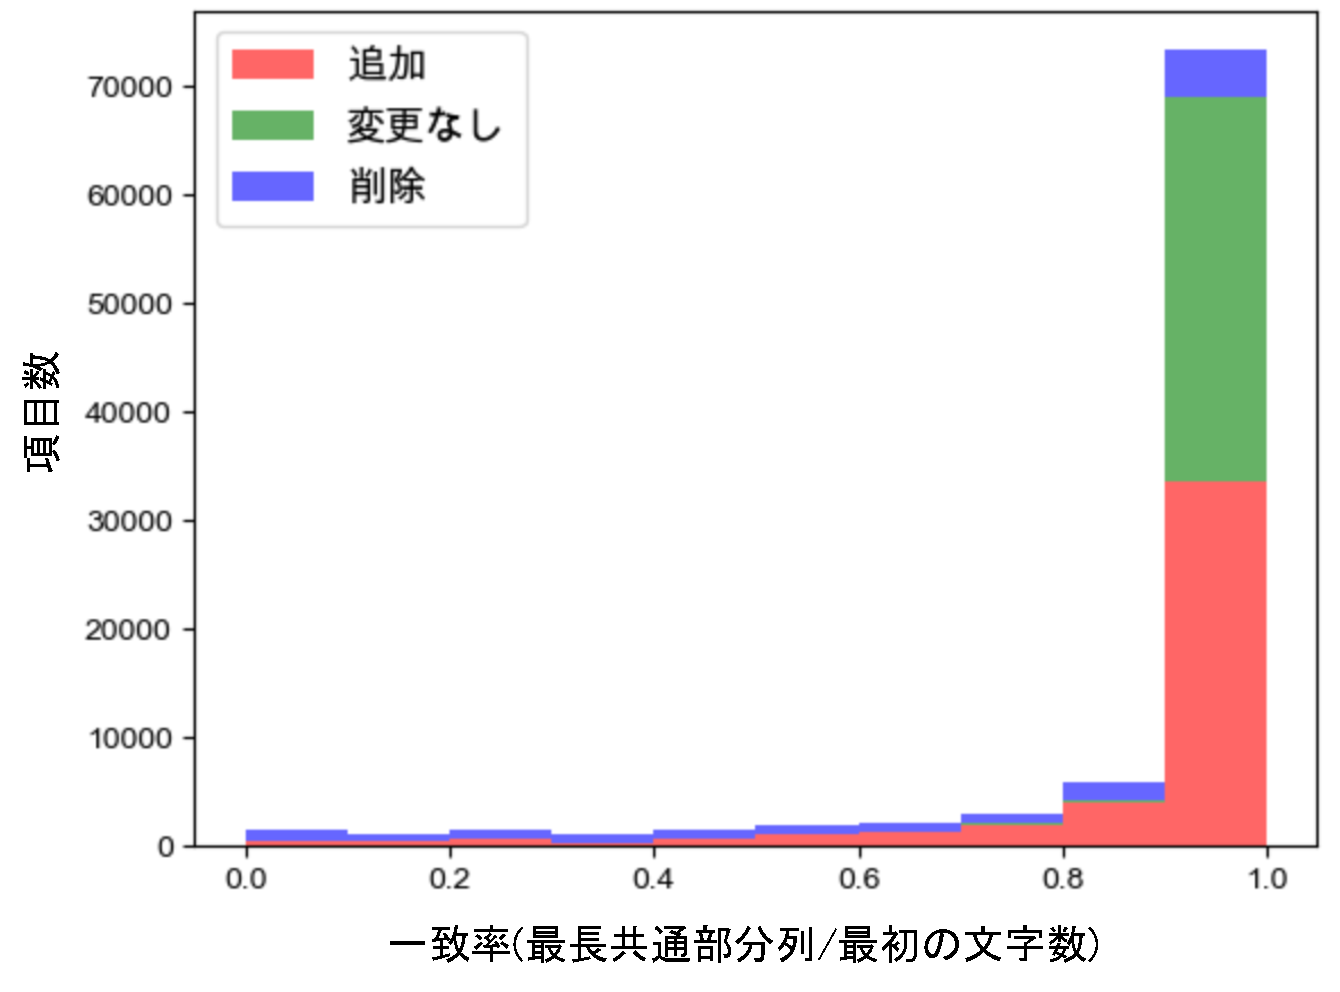
\includegraphics[width=1.0\linewidth]{./IPSJ202303_Ishioka/header_equall2.pdf}
	\caption{同じ項目での比較}
	\label{fig:oss_developments_eq}
\end{figure}
%--------------------------------






%% ーーーーーーーーーーーーーーーー
\subsubsection{異なる項目での比較}
図4.4は初期版と最終版READMEの説明文を異なる項目同士で比較した連続一致率の分布を示す.横軸は連続一致率を表し,縦軸は項目数を表す.連続一致率が高いほど,READMEの変更「細分化」や「統合」が行われる可能性が高いことを示す.結果から,異なる項目において,初期版と最終版READMEの説明文は連続一致率が低く,READMEの変更において「細分化」や「統合」が行われる可能性は低いと示唆される.

%--------------------------------
\begin{figure}[t]
 	\centering
		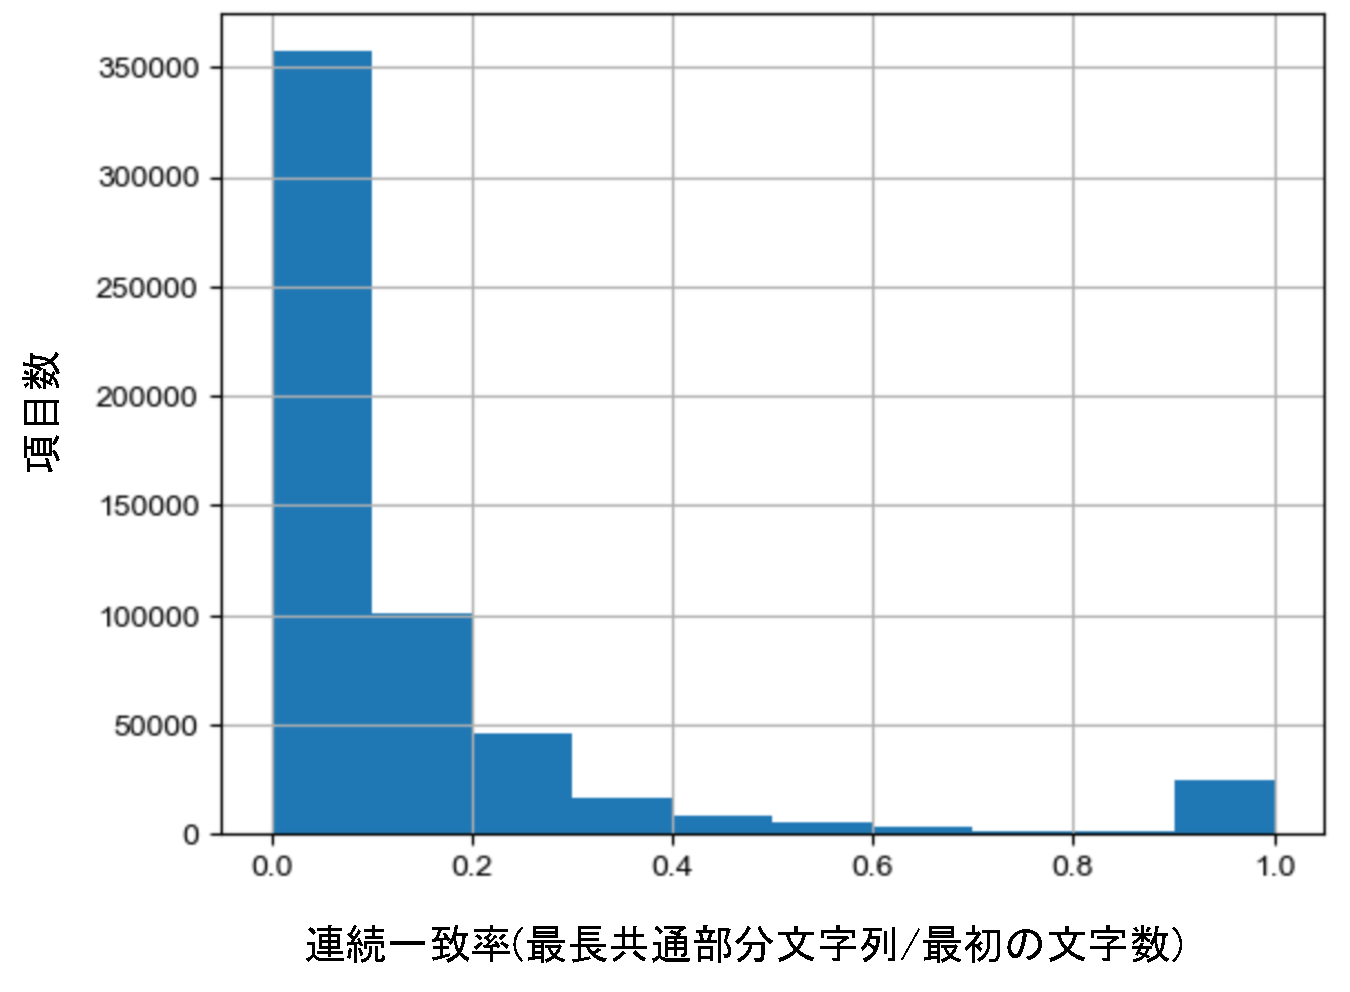
\includegraphics[width=1.0\linewidth]{./IPSJ202303_Ishioka/header_differ2.pdf}
	\caption{異なる項目での比較}
	\label{fig:oss_developments_df}
\end{figure}
%--------------------------------





%% ーーーーーーーーーーーーーーーー
\subsubsection{項目「使用方法」同士の比較}
図4.5は,3章事前分析で適合率が低かった項目「使用方法」同士で比較した一致率の分布を示す.横軸は一致率を表し,縦軸は項目数を表す.一致率が高いほど,READMEの変更「追加」や「削除」が行われる可能性が高いことを示す.赤は初期版と最終版READMEの項目「使用方法」における説明文の一致率が高く,文字数が増加している変更「追加」,緑は初期版と最終版READMEの項目「使用方法」における説明文の一致率が高く,文字数が変化していない「変更なし」,青は初期版と最終版READMEの項目「使用方法」における説明文の一致率が高く,文字数が減少している変更「削除」を表す.結果から,項目「使用方法」においても,初期版と最終版READMEの説明文は一致率が高く,初期版の説明文の内容を基に変更されていた.また,一致率が高い(90-100\%)説明文を確認したところ,9,402件のうち「追加」が行われたのが5,657件,「変更なし」が2,925件,「削除」が行われたのが820件であった.図4.5の結果から,項目「使用方法」においても,README変更において「削除」が行われることは少なく,「追加」が行われることが多いことを確認した.


%--------------------------------
\begin{figure}[t]
 	\centering
		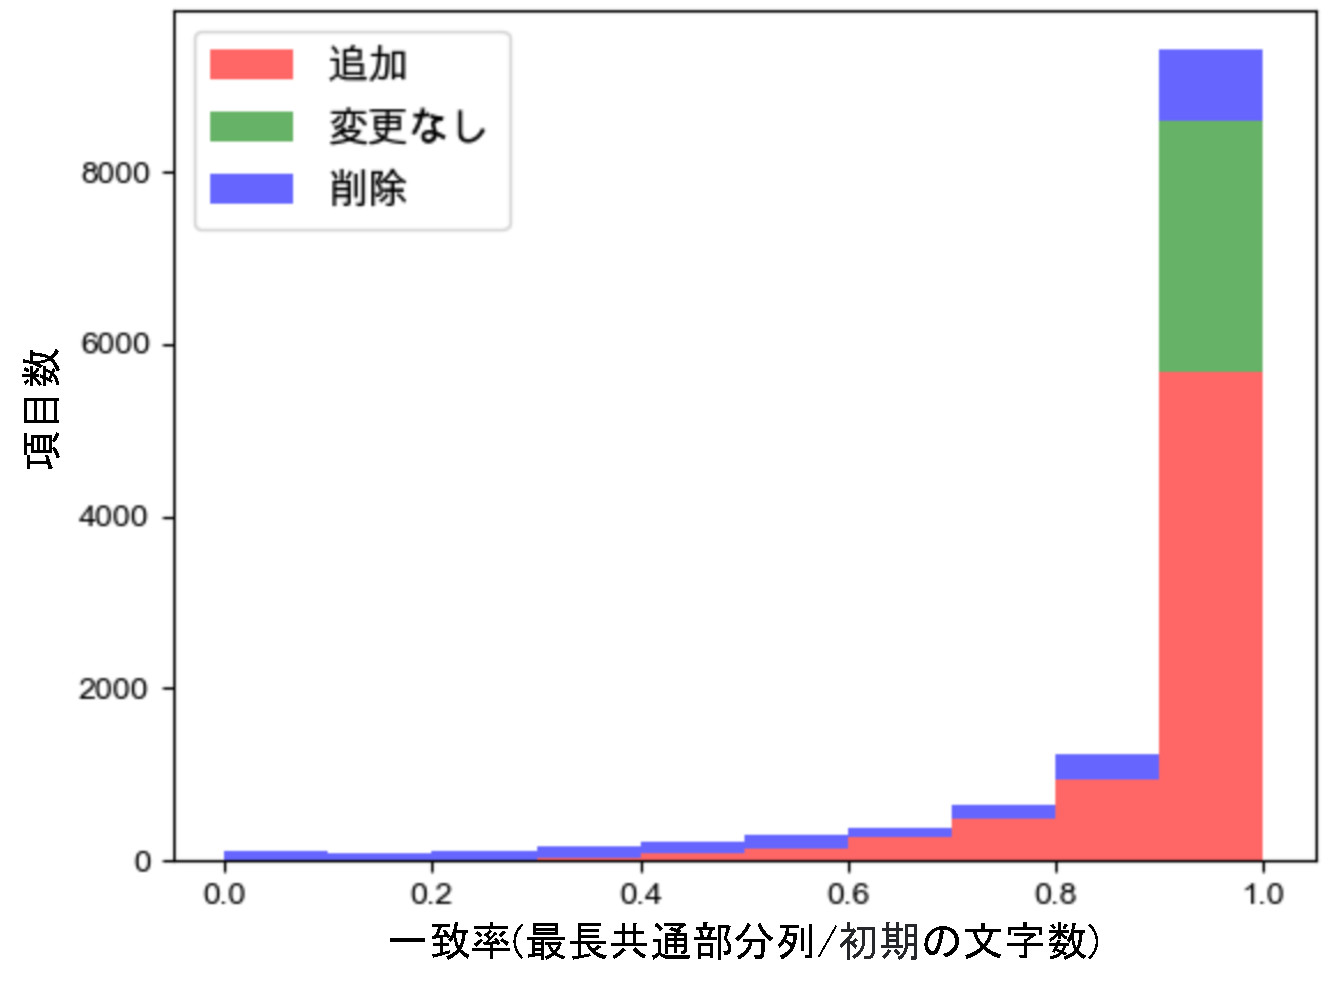
\includegraphics[width=1.0\linewidth]{./IPSJ202303_Ishioka/head_usag_equall2.pdf}
	\caption{項目:使用方法同士での比較}
	\label{fig:oss_developments}
\end{figure}
%--------------------------------






%% ーーーーーーーーーーーーーーーー
\subsubsection{項目「使用方法」と異なる項目の比較}
図4.6から図4.9は,項目「使用方法」の初期版の説明文と3章事前分析で項目「使用方法」と類似する内容が記述される項目「API」,「概要」,「オプション」およびその他項目の最終版の説明文を比較した連続一致率の分布を示す.横軸は連続一致率を表し,縦軸は項目数を表す.連続一致率が高いほど,READMEの変更「細分化」や「統合」が行われる可能性が高いことを示す.3章事前分析の結果から,項目「使用方法」は異なる項目(API,概要,オプション)への説明文の移動を行うことが考えられたが,図4.6から図4.9の結果から,項目「使用方法」においても,READMEの変更において「細分化」や「統合」が行われる可能性は低いと示唆される.
%使用方法に関しては,再現率高かったし,そういう細分化みたいなものの可能性が十分考えられた.それでもなかった〜みたいな風に説明すればいいんじゃない?

分析1の結果から,READMEの変更において,異なる項目への情報の移動は行われず,ソースコードの変更とともに項目ごとに情報を追加していくことを明らかにした.また,本論文で提案する,READMEとその他ファイルの紐付け手法の性能を低下させる要因になる,ソースコードの変更とは無関係なREADMEの変更が行われる可能性が低いことが示唆される.


%分析1の結果から,READMEは初期版では完成されておらず,開発者が必要に応じて,初期版のREADMEの説明文を基に情報を継時的に追加していくことが示唆される.
%結論これでいいの?→懸念していたリファクタリングのような変更はなさそう,項目ごとに追加されていくことが分かった.



%--------------------------------
\begin{figure}[t]
 	\centering
		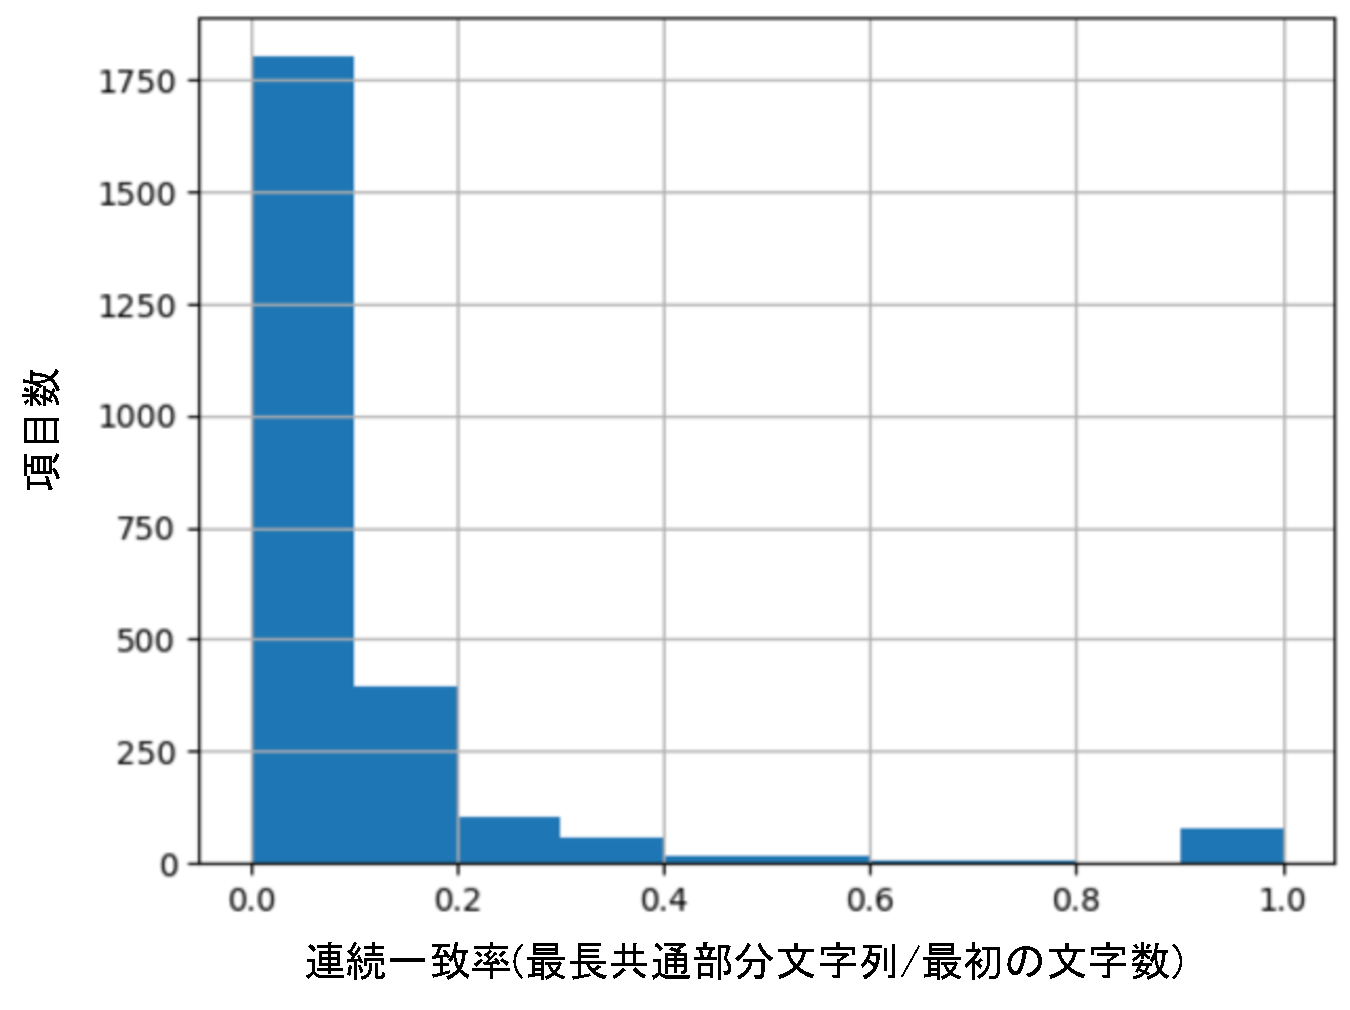
\includegraphics[width=1.0\linewidth]{./IPSJ202303_Ishioka/head_usag_API.pdf}
	\caption{項目:使用方法(初期版)と項目:API(最終版)の比較}
	\label{fig:oss_developments}
\end{figure}
%--------------------------------
\begin{figure}[t]
 	\centering
		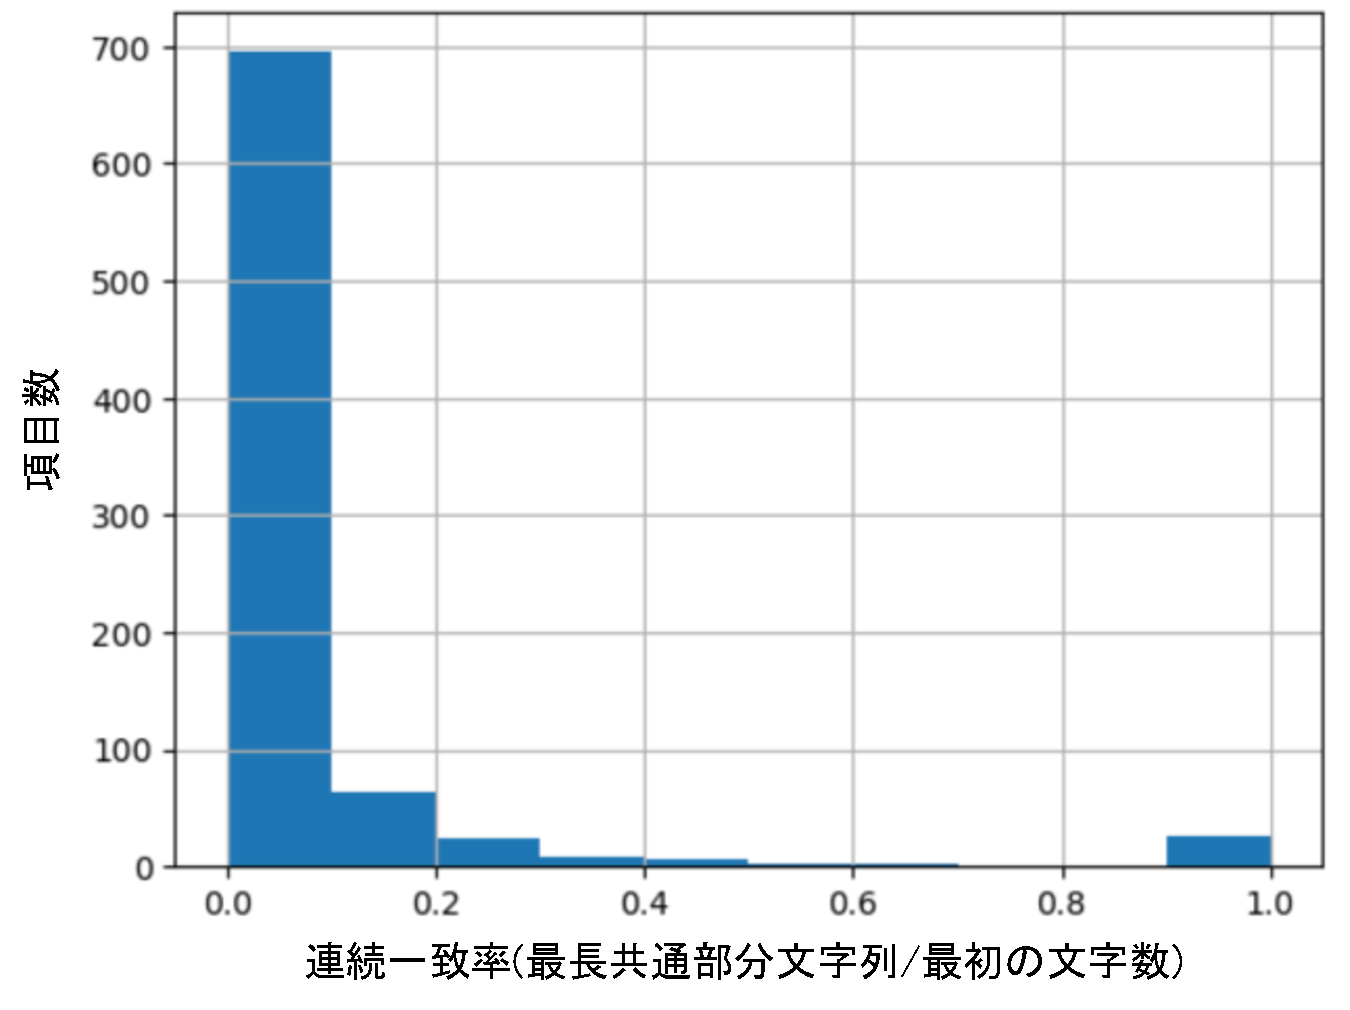
\includegraphics[width=1.0\linewidth]{./IPSJ202303_Ishioka/head_usag_abst.pdf}
	\caption{項目:使用方法(初期版)と項目:概要(最終版)の比較}
	\label{fig:oss_developments}
\end{figure}
%--------------------------------
\begin{figure}[t]
 	\centering
		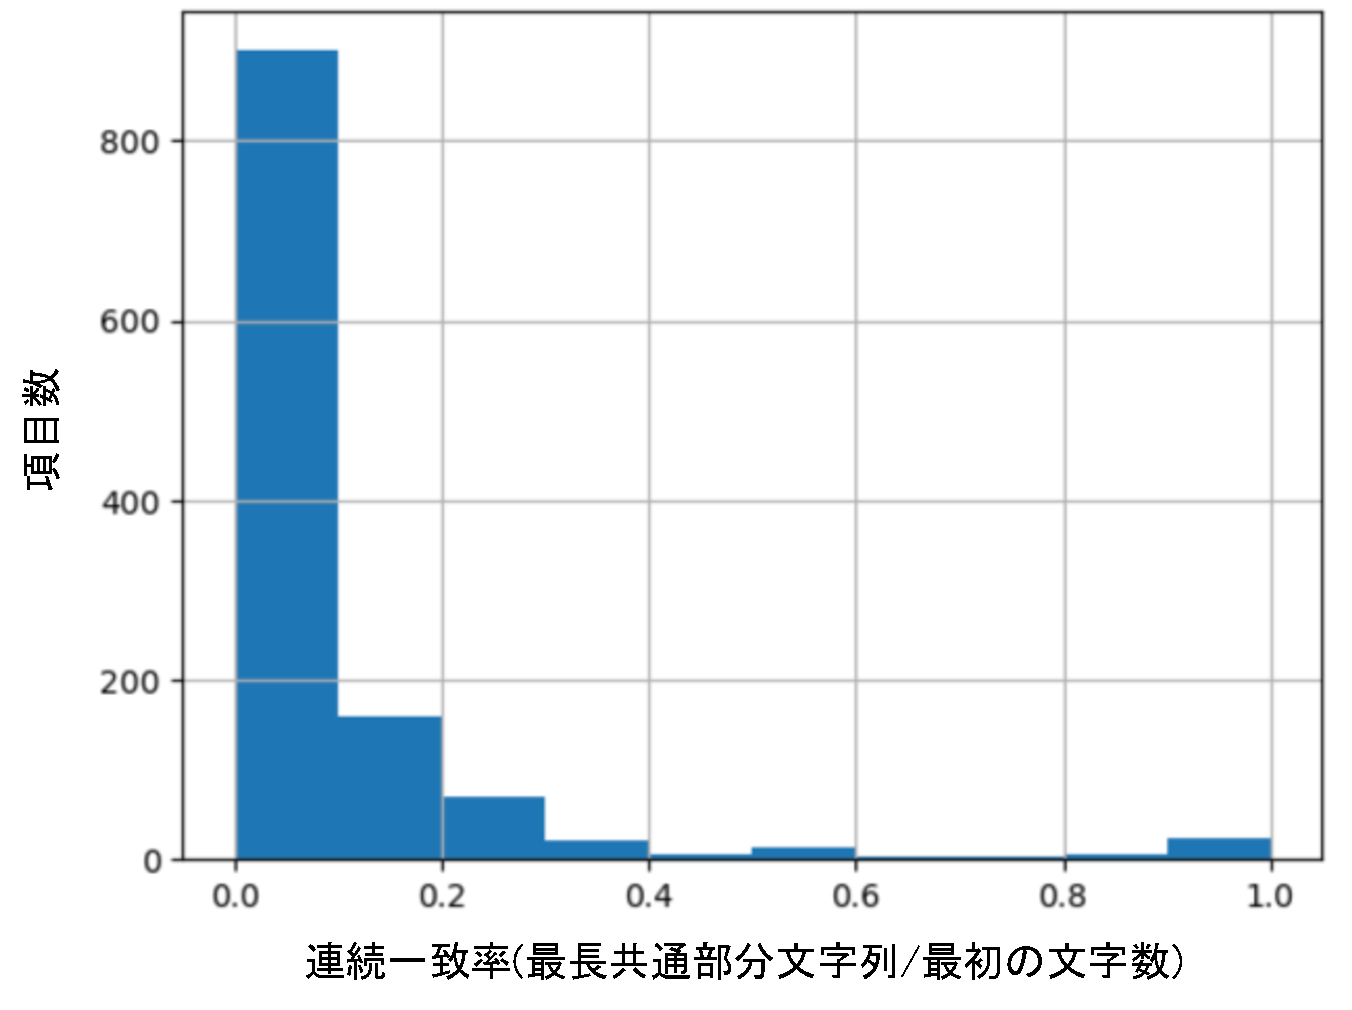
\includegraphics[width=1.0\linewidth]{./IPSJ202303_Ishioka/head_usag_opt.pdf}
	\caption{項目:使用方法(初期版)と項目:オプション(最終版)の比較}
	\label{fig:oss_developments}
\end{figure}
%--------------------------------
\begin{figure}[t]
 	\centering
		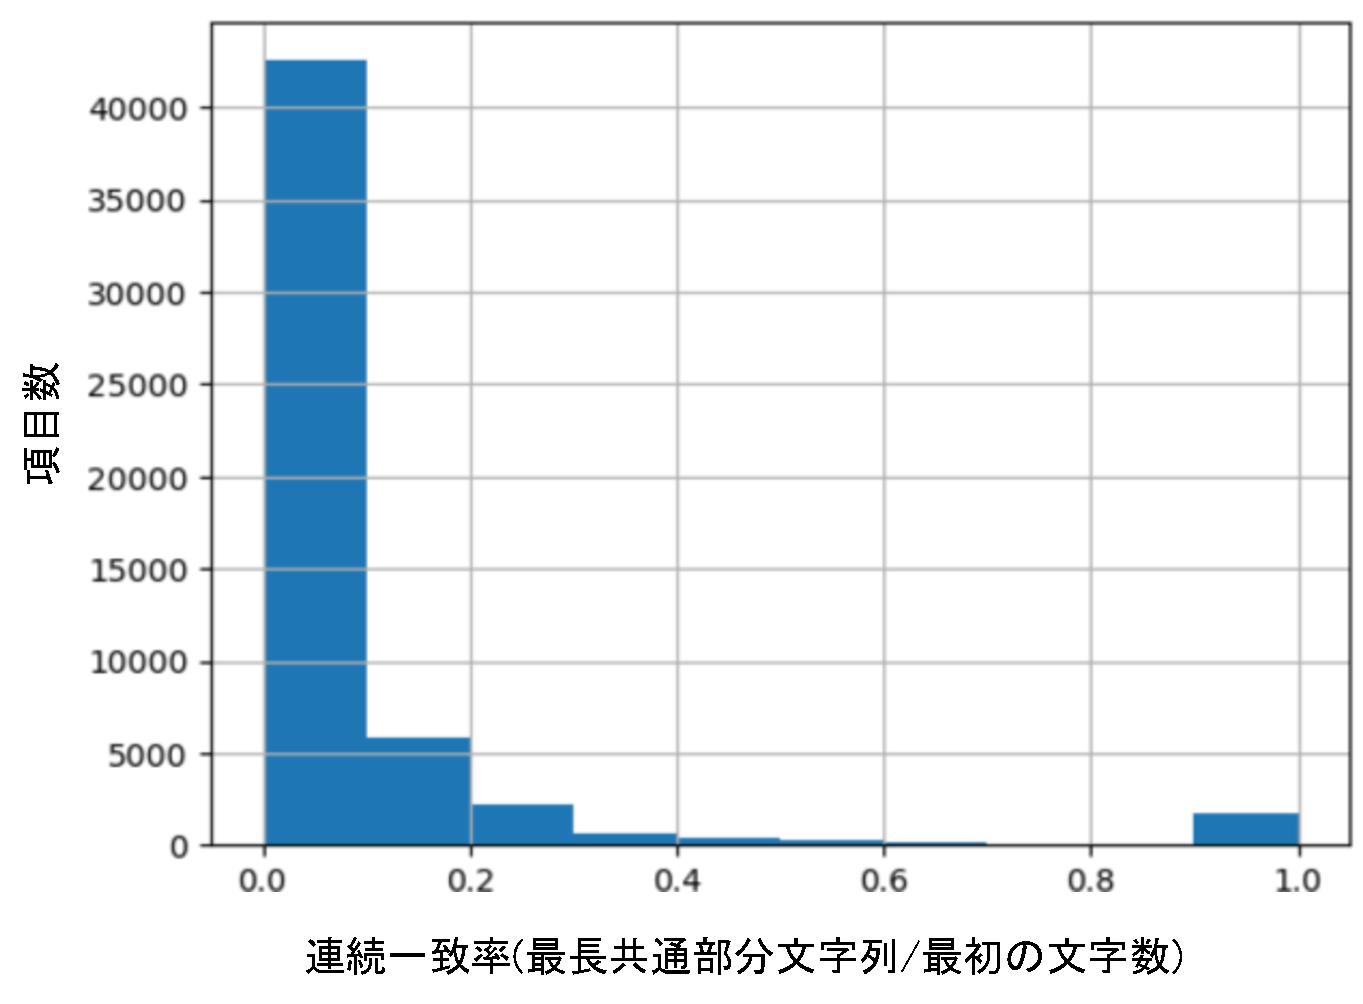
\includegraphics[width=1.0\linewidth]{./IPSJ202303_Ishioka/head_usag_all.pdf}
	\caption{項目:使用方法(初期版)とその他項目(最終版)の比較}
	\label{fig:oss_developments}
\end{figure}
%--------------------------------






%% 5章ーーーーーーーーーーーーーーーーーーーーーーーーーーーーーーーーーーーーーーーーーーーーーーーーーーー
\section{分析2: READMEの変更と紐づくファイルは何か?}

%\textcolor{red}{

%% 5-1ーーーーーーーーーーーーーーーーーーーーーーーーーーーー
\subsection{概要}
%いつ変更するのかというのは,同時に変更されるファイルのタイミングを知ることで解決できる的な話
%紐付けできるか試すために,この研究では,同じ変更意図であることが多い同一コミットに絞り,試すという話

%README変更を開発者に推薦するためには,どのファイルを変更したときにREADMEを変更するのかという情報が必要である.



%同時に変更されるといっても,ほんとに変更内容が共通している(紐づいてる)の?→紐づいてるなら機械的に紐付けできる?紐付けができるなら,どのファイルを変更したときに,RMを変更しないといけないのか推薦できる.的な文章にしたい
%READMEには,新機能の使い方やAPIの説明,オプションの設定方法などの情報が記述されており,その他のファイルの変更に伴って,共にREADMEが変更されることが多い.しかし,同時に変更されたREADMEとその他のファイルの変更意図が共通しているかは明らかではない.本章では,READMEとその他のファイルの変更を機械的に紐付ける手法を提案し,その有用性を評価する.具体的には,READMEの説明文の変更内容とREADMEと同時に変更されたファイルの変更内容を比較し,READMEの変更と紐づくファイルを特定する.READMEの変更とその他のファイルの変更との紐付けができれば,READMEを変更すべきと開発者に推薦することができる.




READMEはソフトウェアの進化に追従して変更されるべきドキュメントであるが,ソースコードを変更するたびにREADMEを変更するとは限らなず,ファイルの変更に合わせて,開発者がREADMEを変更すべきか判断が困難であるため,開発者はREADMEの変更を見落とすと考えられる.開発者のREADME変更の作業負荷を低減させ,ソースコードの変更とともにREADMEが変更されるようにするためには,READMEの変更と直接関係があるファイルを把握する必要がある.

READMEには,新機能の使い方やAPIの説明,オプションの設定方法などの情報が記述されており,その他のファイルの変更に伴って,共にREADMEが変更されることが多い.しかし,同時に変更されたREADMEとその他のファイルの変更意図が共通しているかは明らかではない.READMEと同時に変更されるファイルのうち,READMEと変更意図が一致するファイルは,すぐにその変更内容をREADMEに反映した(READMEの変更と直接関係があるファイルである)と考え,本論文では,同時に変更されたREADMEとファイルを対象とする.本章では,READMEとその他のファイルの変更を機械的に紐付ける手法を提案し,その有用性を評価する.具体的には,READMEの説明文の変更内容とREADMEと同時に変更されたファイルの変更内容を比較し,READMEの変更と紐づくファイルを特定する.本論文で提案するREADMEとその他のファイルの紐付け手法によって,変更意図が一致するREADMEの変更とその他のファイルの変更を機械的に紐付けできれば,開発者のファイル変更に合わせて,README変更を開発者に推薦することで,開発者のREADME変更支援やREADMEを常に最新の状態にするといったREADMEの品質向上につながることを期待する.





%% 5-2ーーーーーーーーーーーーーーーーーーーーーーーーーーーー
\subsection{データセット}
\subsubsubsection{コミットの抽出}
3章の事前分析および4章の分析1同様に,52,292件のプロジェクトのREADMEを分析対象とする.同時に変更されたREADMEとその他のファイルの変更意図が共通しているか確認するために,52,292件のプロジェクトのREADMEの変更履歴からREADMEが変更されたコミットを抽出する.その結果,得られた184,598コミットをデータセットとして使用する.

\subsubsubsection{評価用データの作成}
本章では,同時に変更されたREADMEの説明文の変更内容とその他のファイルの変更内容を比較し,機械的にREADMEの変更と紐づくファイルを特定する.正しく特定できているかを評価するために,データセットからランダムに抽出したコミットを目視で確認し,評価用データの作成を行う.具体的には,データセットからランダムに抽出した384コミット(信頼区間95\%,信頼度±5\%)で変更されたREADMEおよびファイルの変更内容およびコミットメッセージを目視で確認し,READMEとファイルの変更意図が同じであるか否かを分類する.


%% 5-3ーーーーーーーーーーーーーーーーーーーーーーーーーーーー
\subsection{手法}
本章では,同時に変更されたREADMEの説明文の変更内容とその他のファイルの変更内容を比較し,機械的にREADMEの変更と紐づくファイルを特定する.特定は次の手順で行う.
%--------------------------------
\subsubsection{手順1:変更差分の抽出}
コミットからREADMEおよびファイルの変更差分の抽出を行う.分析1の結果より,READMEの変更において情報の追加が行われることがわかった.本論文ではREADMEの変更と紐づくファイルを特定するため,READMEおよびファイルの変更内容のうち,削除された部分ではなく追加された部分を対象とし,追加された行を変更差分として抽出する.
%--------------------------------
\subsubsection{手順2:モデル構築}
手順1で抽出したREADMEおよびファイルの変更差分を入力として,READMEとファイルの変更意図が一致するか否かの2クラス分類モデルの構築を行う.モデルの構築には自然言語処理分野でよく使用されるBag of Words (BoW)とBERTに加え,CodeBERTを用いる.

 \begin{itemize}
    \item Bag of Words (BoW): 自然言語で記述された文書に含まれる単語を出現回数に基づきベクトル表現を得る.BoWはシンプルで理解しやすいが,単語の順序や文脈を考慮していないため,文の意味の一部が失われる可能性がある.

    \item BERT\cite{BERT}: 自然言語処理のタスクにおいてよく使用される事前学習モデル.Transformer\cite{Transfomer}ベースのモデルであり,双方向の文脈を考慮している.大量のテキストデータで事前学習され,単語の文脈に基づいた豊富なベクトル表現を得る.本論文では,一般的に使用される標準的なモデルHugging Face Transformersの事前学習モデル「bert-base-uncased」を使用する.
  \end{itemize}

変更差分には,自然言語だけでなくソースコードも含まれるため,自然言語だけでなく複数のプログラム言語のコーパスを用いて事前学習されたCodeBERTも用いる.

 \begin{itemize}
    \item CodeBERT\cite{CodeBERT}: プログラムに特化したBERTベースのモデル.RoBERTa\cite{RoBERTa}をベースにしており,プログラミング関連のタスクに適したベクトル表現を獲得.大規模なプログラムと自然言語のペアのデータセットで事前学習される.事前学習には,CodeSerchNet\cite{CodeSerchNet}から収集された6言語(Ruby,JavaScript,Go,Python,Java,PHP)のメソッドとコメントのペアが用いられ,コード分類やコード要約,ドキュメント生成などで高い性能を発揮する.CodeBERTは,プログラムの文脈を理解し,自然言語とプログラムの間の意味的な関係を捉えることができる.本論文では,Hugging Face Transformersの事前学習モデル「codebert-base」を使用する.
 \end{itemize}


BoW,BERTおよびCodeBERTのモデル構築方法について順に記述する.

\subsubsubsection{BoWモデル}
ベクトル間の類似度が任意の閾値以上の場合に,READMEの変更内容とその他のファイルの変更内容を機械的に紐付けられると考え,READMEとファイルの変更意図が一致するか否かの2クラス分類モデルを構築する.具体的には,手順1で抽出した変更差分に対して,BoWを用いてベクトル化を行う.次に,READMEの変更とその他ファイルの変更内容が一致するのか確認するために,類似度を算出する.類似度の算出には,一般的にベクトル表現の類似度算出に使用されるコサイン類似度を用いる.算出した類似度が閾値以上であればREADMEとファイルの変更意図が一致する,閾値未満であれば一致しないと分類する.

\subsubsubsection{BERTモデルおよびCodeBERTモデル}
事前学習されたBERTおよびCodeBERTをファインチューニングし,READMEとファイルの変更意図が一致するか否かの2クラス分類を行うモデルの構築を行う.具体的には,BERTおよびCodeBERTの最後に全結合層(線形)を追加する.次に,手順1で抽出したREADMEおよびファイルの変更差分を入力として与え,READMEとファイルの変更意図が一致するか否か(0または1)を出力させる.図5.1はモデルの構成図を示す.5章2節で作成した評価用データからランダムに8割抽出し,ファインファインチューニングに用いる.残りの2割のデータを用いて,モデルの評価を行う.また,今回使用するBERTの事前学習モデル「bert-base-uncased」およびCodeBERTの事前学習モデル「codebert-base」の最大入力トークン長が512であるため,READMEおよびファイルの変更差分が512を超える場合は,512トークン分までを入力として用いる.

%-------------------------
\begin{figure}[t]
 	\centering
		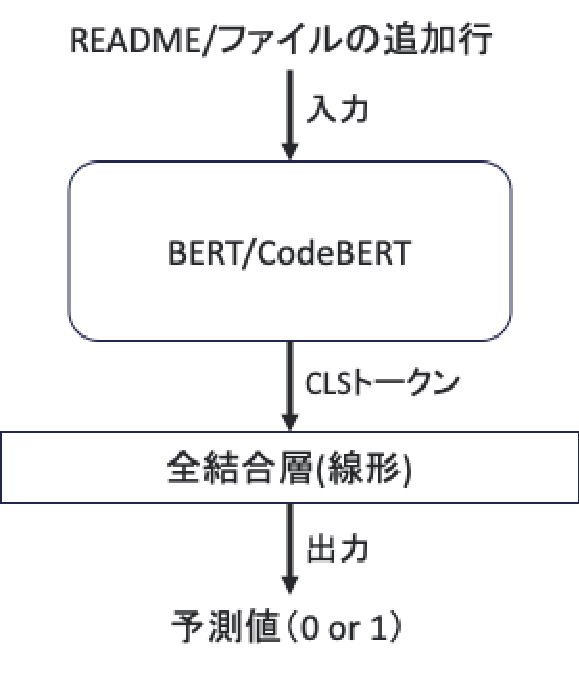
\includegraphics[width=0.4\linewidth]{./IPSJ202303_Ishioka/BERT_flow.pdf}
	\caption{BERTモデルおよびCodeBERTモデルの構成図}
	\label{fig:oss_developments}
\end{figure}
%-------------------------

%--------------------------------
\subsubsection{手順3:評価}
手順2で各モデルが出力した結果が評価用データと一致しているかを確認するために,評価指標の値を比較する.評価指標には,適合率,再現率,F1値を用いる.また,BoWモデルは閾値によって評価結果が異なるため,AUC-ROC(Area Under the Curve - Receiver Operating Characteristic)を使用する.AUC-ROCは確率的な閾値に依存する適合率や再現率とは異なり,すべての可能な閾値を考慮する閾値に依存しない評価方法である.


%上記手順で算出した類似度が任意の閾値以上の場合に,READMEの変更内容がその他のファイルの変更内容と機械的に紐付けられると考え,READMEと変更意図が一致するか否かの2クラス分類を行う.手法の類似度が評価用データと一致しているかを確認するために,評価指標の値を比較する.評価指標には,適合率,再現率,F1値,AUC-ROC(Area Under the Curve - Receiver Operating Characteristic)を使用する.AUC-ROCは確率的な閾値に依存する適合率や再現率とは異なり,すべての可能な閾値を考慮する閾値に依存しない評価方法である.



%% 5-4ーーーーーーーーーーーーーーーーーーーーーーーーーーーー
\subsection{結果}
表5.1は目視の結果得られたREADMEの変更と変更意図が一致するファイル数を示す.ランダムに抽出した384コミットから1,553件のファイルの変更差分が得られた.得られた1,553件のファイルの変更差分を評価用データとして用いて分析を行う.

表5.2は,得られたファイルおよび拡張子数の上位5件を示す.本論文では,JavaScript言語を用いたプロジェクトを対象としているため,「.js」および「.json」ファイルが他拡張子よりも多くREADMEと同時に変更されている.また,自然言語で記述されることの多い「.md」ファイルが「.js」および「.json」ファイルに次いで,READMEと同じコミットで多く変更されている.データセットから,READMEはプログラムファイルだけでなく同じ自然言語で記述されるファイルと同時に変更されていることがわかる.





%BoW_test_AUC.pdf
%BoW_test_PR.pdf
%BoW_testdata.pdf





%\begin{itemize}
%  \item 全てのファイル: 全てのファイル(1,553件)を対象に,READMEの変更と紐づくファイルを特定する.
%  \item プログラムファイルのみ : プログラムファイルのみ(1,127件)を対象に,READMEの変更と紐づくファイルを特定する.プログラム言語に特化した手法であるCodeBERT,CodeT5+が,他の手法よりも精度が高いことが考えられる.
%\end{itemize}
%
%\subsection{全てのファイルの結果}
%表5.2は,得られたファイルおよび拡張子数の上位5件を示す.本論文では,JavaScript言語を用いたプロジェクトを対象としているため,「.js」および「.json」ファイルが他拡張子よりも多くREADMEと同時に変更されている.また,自然言語で記述されることの多い「.md」ファイルが「.js」および「.json」ファイルに次いで,READMEと同じコミットで多く変更されている.データセットから,READMEはプログラムファイルだけでなく同じ自然言語で記述されるファイルと同時に変更されていることがわかる.

%--------------------------------
\begin{table}[t]
 \centering
 \caption{評価用データ}
\label{tab:result}
  \scalebox{1.0}{
  \begin{tabular}{l|r} 
  \hline\hline
     & ファイル数\\\hline 
    READMEと変更意図が一致する(正解) & 781件\\
    \hline 
    READMEと変更意図が一致しない(不正解) & 772件\\
    \hline 
    合計 & 1,553件\\ \hline
  \end{tabular}
    \label{tab:result}
   }
\end{table}
%--------------------------------

%--------------------------------
\begin{table}[t]
  \caption{READMEと同時に変更されたファイル名/拡張子上位5件}
  \centering
  \begin{tabular}{l|rll|r}
%\hline
    \cline{1-2}\noalign{\vspace{1pt}}\cline{1-2}\cline{4-5}\noalign{\vspace{1pt}}\cline{4-5}
    ファイル名 & ファイル数 && 拡張子 & 拡張子数\\
    \cline{1-2}\cline{4-5}
    package.json       & 235 && js & 738\\
    index.js           & 119 && json & 295\\
    CHANGELOG.md       & 54 && md & 101\\
    index.html         & 34 && ts & 69\\
    package-lock.json  & 26 && html & 60\\
    \cline{1-2}\cline{4-5}
  \end{tabular}

  % \begin{tabular}{l|r}
  %   \hline\hline
  %   拡張子 & 拡張子数\\
  %   \hline
  %   js    & 738 \\
  %   json  & 295 \\
  %   md    & 101 \\
  %   ts    & 69 \\
  %   html  & 60 \\
  %   \hline
  % \end{tabular}

  \label{tab:file_comparison}
\end{table}
%--------------------------------

%--------------------------------
\begin{figure}[t]
 	\centering
		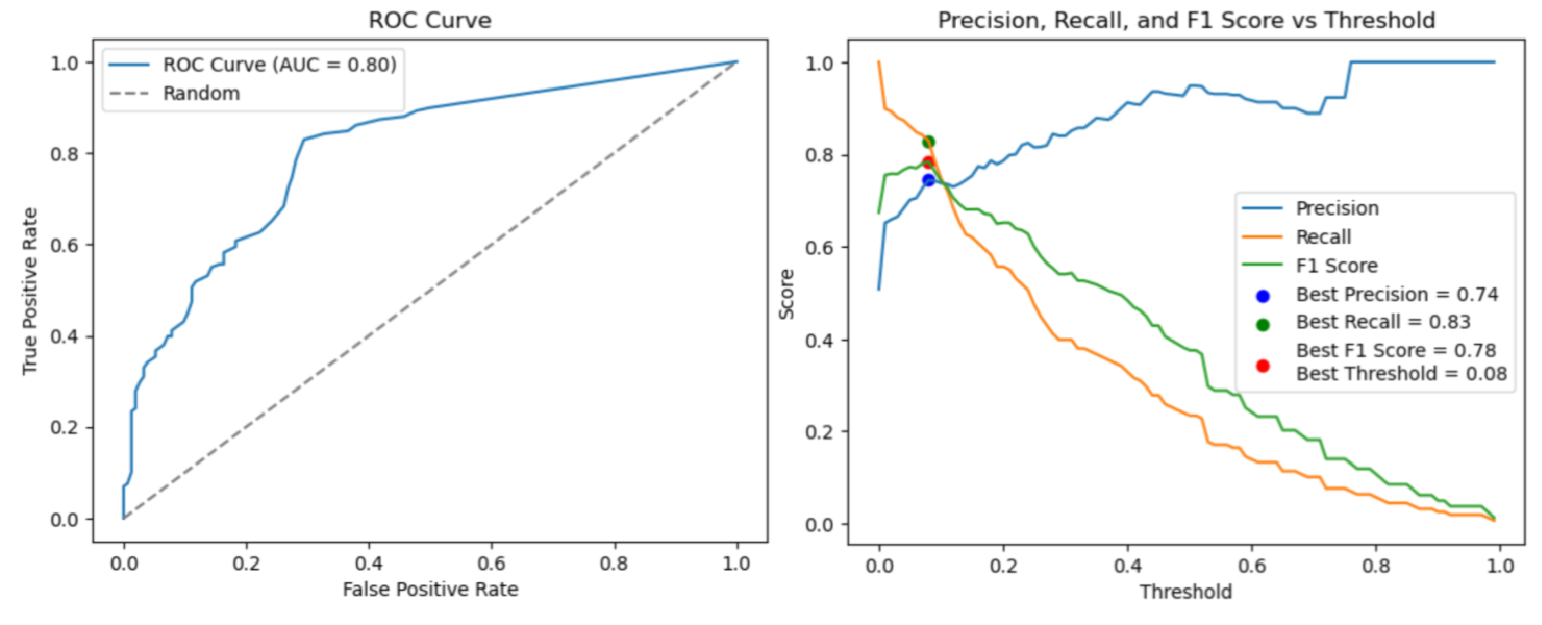
\includegraphics[width=1.0\linewidth]{./IPSJ202303_Ishioka/BoW_testdata.pdf}
	\caption{Bag-of-Wordsでの結果}
        \ecaption{hoge}
	\label{fig:oss_developments}
\end{figure}
%--------------------------------

%%--------------------------------
%\begin{figure}[t]
% 	\centering
%		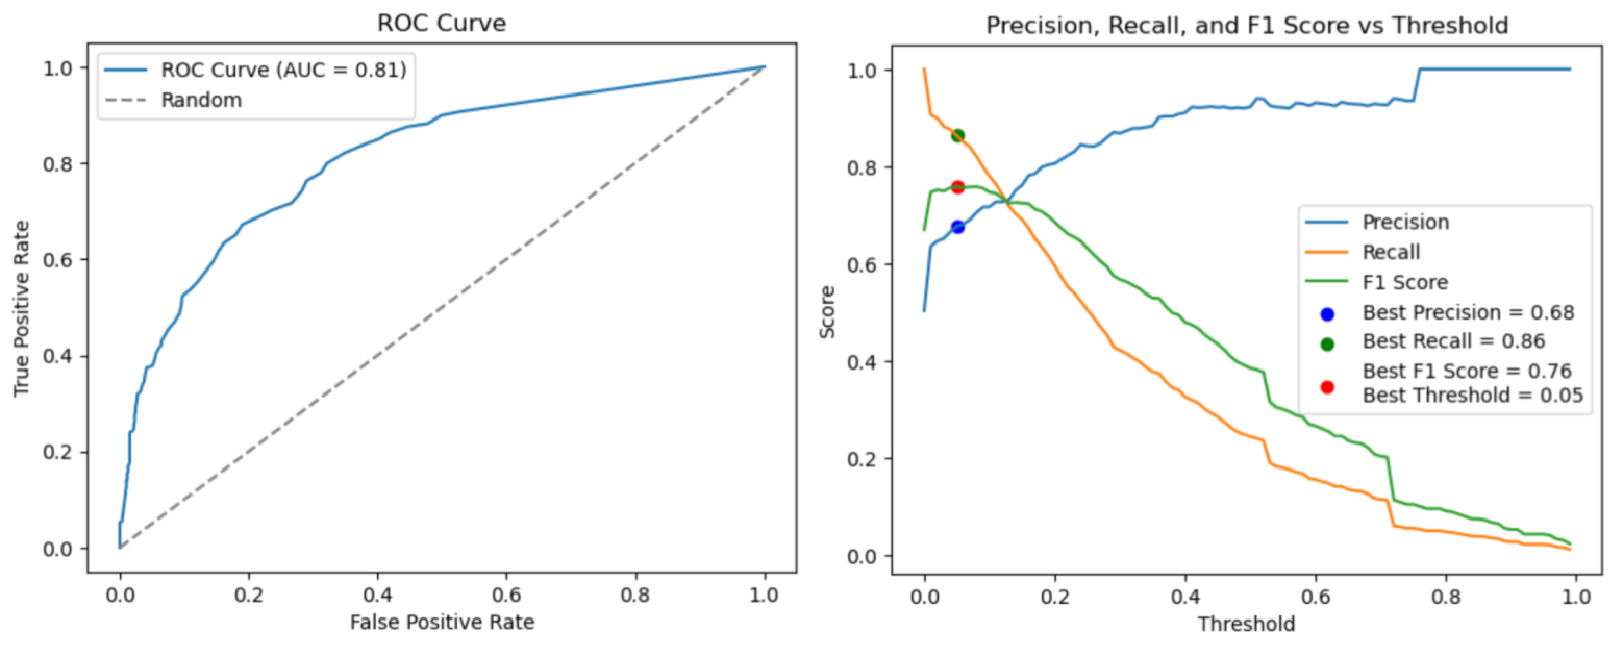
\includegraphics[width=1.0\linewidth]{./IPSJ202303_Ishioka/BoW.pdf}
%	\caption{Bag-of-Wordsでの結果}
%	\label{fig:oss_developments}
%\end{figure}
%%--------------------------------
%\begin{figure}[t]
% 	\centering
%		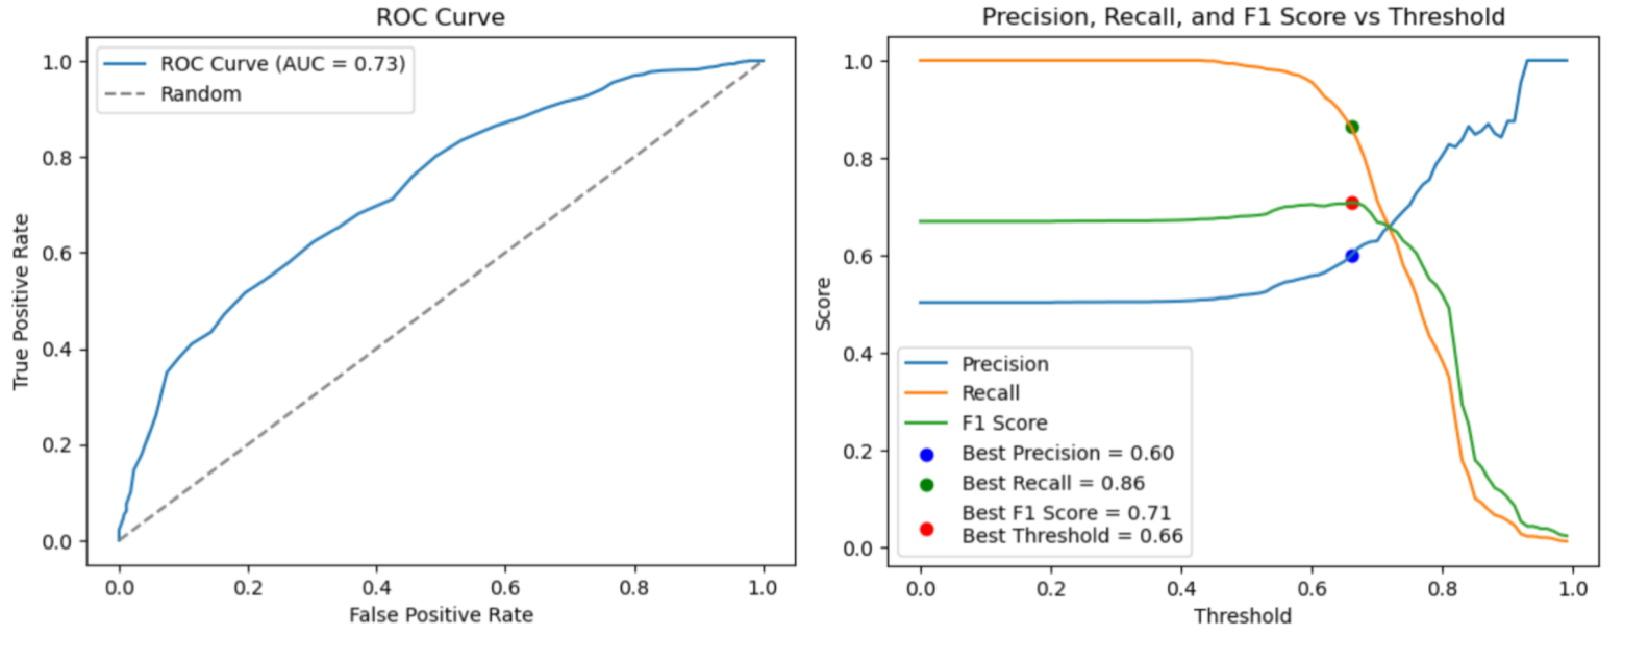
\includegraphics[width=1.0\linewidth]{./IPSJ202303_Ishioka/BERT.pdf}
%	\caption{BERTでの結果}
%	\label{fig:oss_developments}
%\end{figure}
%%--------------------------------
%\begin{figure}[t]
% 	\centering
%		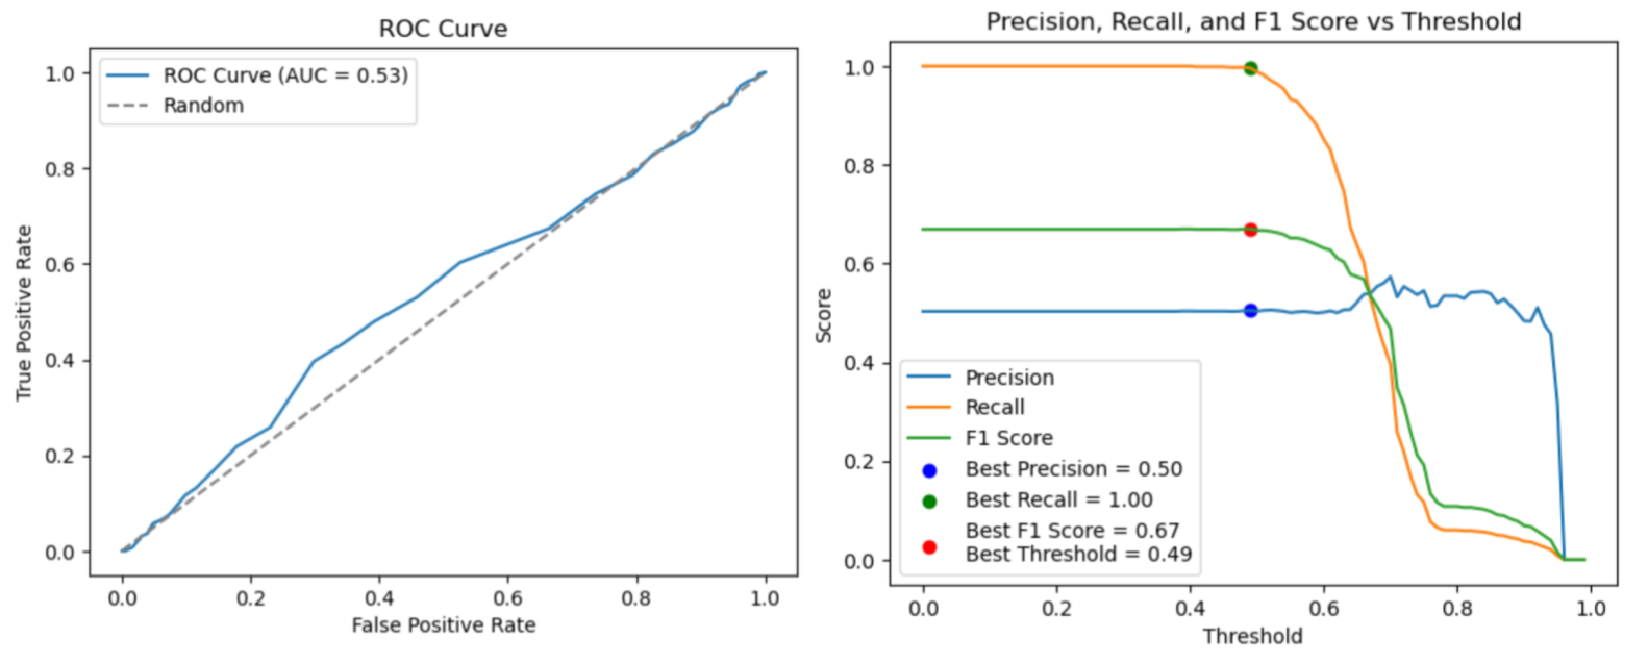
\includegraphics[width=1.0\linewidth]{./IPSJ202303_Ishioka/CodeBERT.pdf}
%	\caption{CodeBERTでの結果}
%	\label{fig:oss_developments}
%\end{figure}
%%--------------------------------
%\begin{figure}[t]
% 	\centering
%		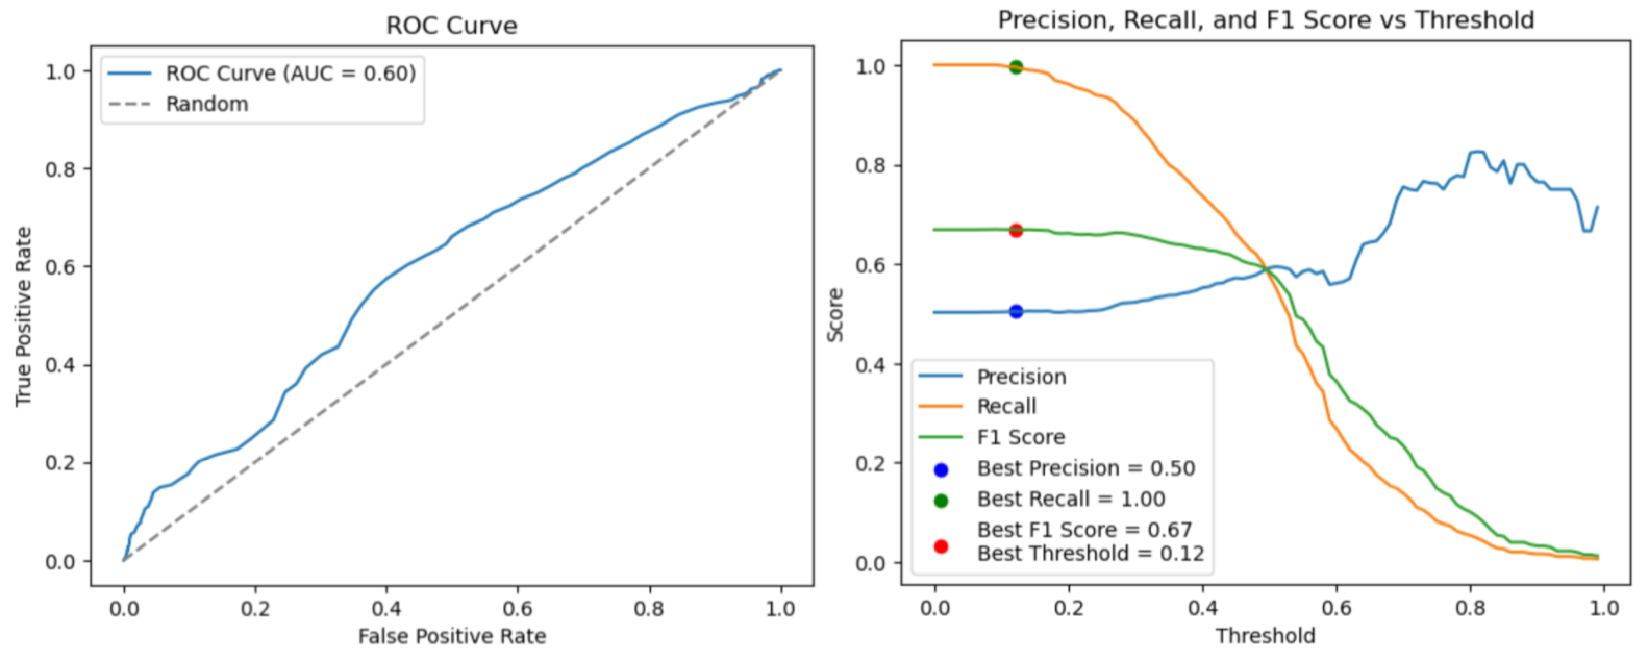
\includegraphics[width=1.0\linewidth]{./IPSJ202303_Ishioka/CodeT5.pdf}
%	\caption{CodeT5+での結果}
%	\label{fig:oss_developments}
%\end{figure}
%%--------------------------------



図5.2の左図は,BoWのROC(Receiver Operating Characteristic)曲線を表す.ROC曲線は2クラス分類の性能を評価するためのグラフで,横軸は偽陽性率(実際にはREADMEの変更意図と一致しないファイルを,一致すると誤分類した割合),縦軸は真陽性率(実際にREADMEの変更意図と一致するファイルを,正しく一致すると分類できた割合)を示す.ROC曲線が左上隅に近い凸型で,AUC(曲線下面積)の値が大きいほど性能が高く,READMEとファイルを紐付けられていると解釈する.図5.2の右図は,BoWの閾値ごとの適合率,再現率,F1値の変化を表す.横軸は閾値,縦軸は適合率,再現率,F1値の結果を示す.BERTおよびCodeBERTの結果と比較するために,BoWの結果は,図5.2の右図において最も性能が高かった値を用いる.

表5.3は各手法の適合率,再現率,F1値の結果を示す.
適合率においては,BERT(適合率=0.91),CodeBERT(適合率=0.86),BoW(適合率=0.74)の順で,BERTが最も良い結果となった.
BERTおよびCodeBERTがBoWよりも高い適合率を示していることから,自然言語の文脈を考慮することで,より正確な分類が可能になることが示唆される.また,1つの単語だけでなく複数単語で構成される専門用語をフレーズとして扱うことができたため,高い適合率を示したと考えられる.
再現率においては,BoW(再現率=0.83),CodeBERT(再現率=0.76),BoW(再現率=0.67)の順で,BoWが最も良い結果となった.
BoWは単語の出現頻度に基づくモデルであり,一般的な特徴を捉えやすい.BoWが最も高い再現率を示していることから,固有名詞や関数名などの有無が性能に強く寄与していることが示唆される.また,BERTの再現率が他と比較して低くなっている原因として,BERTの事前学習で行われるサブワード分割が,一般的なドキュメントを前提としているため,低くなったと考えられる.一方でCodeBERTはプログラムに使用されるフレーズなどを考慮できたため,BERTよりも高い再現率を示したと考えられる.
F1値においては,CodeBERT(F1値=0.81),BERT(F1値=0.78),BoW(F1値=0.77)の順で,CodeBERTが最も良い結果となった.CodeBERTは自然言語およびプログラムの文脈を考慮することで,適合率と再現率の両方で良好な性能を示している.このことから,自然言語とプログラムの文脈も考慮することで,コードに特化したトークン化や埋め込み表現によりプログラムの特徴を捉えることができ,READMEとその他のファイルの紐付け性能の向上につながったと考えられる.

分析2の結果から,文脈を考慮することが全ての指標において最適であるわけではないが,自然言語やプログラムの文脈を考慮することで,モデルの性能向上につながることが明らかとなった.


%また,BERTの再現率が他と比較して低くなっている原因として,BERTの事前学習で行われるサブワード分割が,一般的なドキュメントを前提としているため,低くなったと考えられる.一方でCodeBERTはプログラムに使用されるフレーズなどを考慮できたため,BERTよりも高い再現率を示したと考えられる.
%また,BERTの再現率が他と比較して低くなっている原因として,文脈を考慮することによって,固有名詞や関数名などの有無といった情報の重要度が下がってしまい,正例を見逃してしまった可能性が考えられる.
%
%複数のプログラム言語のコーパスを用いて事前学習されたCodeT5+およびCodeBERTよりも,プログラム言語のコーパスで事前学習をしていないBoWおよびBERTの方が高い性能を発揮した.この結果については考察で述べる.
%分析2の結果から,READMEとその他のファイルの紐付けを行う上で,プログラム言語の文脈を考慮して変更差分のベクトル化を行うよりも,変更差分に含まれる自然言語が重要であることが示唆される.



%--------------------------------
\begin{table}[t]
  \centering
  \caption{各手法の適合率,再現率,F1値}
  \ecaption{hoge}
    \begin{tabular}{l|r|r|r}\hline\hline
    手法 & 適合率 & 再現率 & F1値 \\\hline
    BoW & 0.74 & \underline{\textbf{0.83}} & 0.78 \\
    BERT  & \underline{\textbf{0.91}} & 0.67 & 0.77 \\
    CodeBERT & 0.86 & 0.76 & \underline{\textbf{0.81}} \\\hline
    \end{tabular}
  \label{tab:performance_metrics}
\end{table}
%--------------------------------





%図5.1から図5.4の左図は,各手法のROC(Receiver Operating Characteristic)曲線を表す.ROC曲線は2クラス分類の性能を評価するためのグラフで,横軸は偽陽性率(実際にはREADMEの変更意図と一致しないファイルを,一致すると誤分類した割合),縦軸は真陽性率(実際にREADMEの変更意図と一致するファイルを,正しく一致すると分類できた割合)を示す.ROC曲線が左上隅に近い凸型で,AUC(曲線下面積)の値が大きいほど性能が高く,READMEとファイルを紐付けられていると解釈する.
%
%図5.1から図5.4の右図は,各手法の閾値ごとの適合率,再現率,F1値の変化を表す.横軸は閾値,縦軸は適合率,再現率,F1値の結果を示す.図5.1はBoWでの結果,図5.2はBERTでの結果,図5.3はCodeBERTでの結果,図5.4はCodeT5+での結果を示す.ROC曲線の結果から性能は,BoW(AUC=0.81),BERT(AUC=0.73),CodeT5+(AUC=0.60),CodeBERT(AUC=0.53)の順となった.また,F1値の最大値の結果から,BoW(F1=0.76),BERT(F1=0.71),CodeT5+(F1=0.67),CodeBERT(F1=0.67)の順となった.表5.2より,拡張子が「js」や「json」といったプログラムファイルが変更ファイルの半数以上を占めているにも関わらず,複数のプログラム言語のコーパスを用いて事前学習されたCodeT5+およびCodeBERTよりも,プログラム言語のコーパスで事前学習をしていないBoWおよびBERTの方が高い性能を発揮した.この結果については考察で述べる.




%%--------------------------------
%\subsection{プログラムファイルのみの結果}
%プログラムファイルにおける各手法の影響を比較するために,プログラムファイルのみを対象に各手法でベクトル化を行った結果を図5.5から図5.8に示す.図5.5はBoWでの結果(プログラムファイルのみ),図5.6はBERTでの結果(プログラムファイルのみ),図5.7はCodeBERTでの結果(プログラムファイルのみ),図5.8はCodeT5+での結果(プログラムファイルのみ)を示す.ROC曲線の結果から性能は,BoW(AUC=0.79),BERT(AUC=0.71),CodeT5+(AUC=0.60),CodeBERT(AUC=0.52)の順となった.また,F1値の最大値の結果から,BoW(F1=0.76),BERT(F1=0.72),CodeT5+(F1=0.69),CodeBERT(F1=0.68)の順となった.拡張子が「js」や「json」といったプログラムファイルのみを対象に行った結果も,複数のプログラム言語のコーパスを用いて事前学習されたCodeT5+およびCodeBERTよりも,プログラム言語のコーパスで事前学習をしていないBoWおよびBERTの方が高い性能を発揮した.この結果については考察で述べる.
%
%
%
%分析2の結果から,READMEとその他のファイルの紐付けを行う上で,プログラム言語の文脈を考慮して変更差分のベクトル化を行うよりも,変更差分に含まれる自然言語が重要であることが示唆される.
%
%
%
%%--------------------------------
%\begin{figure}[t]
% 	\centering
%		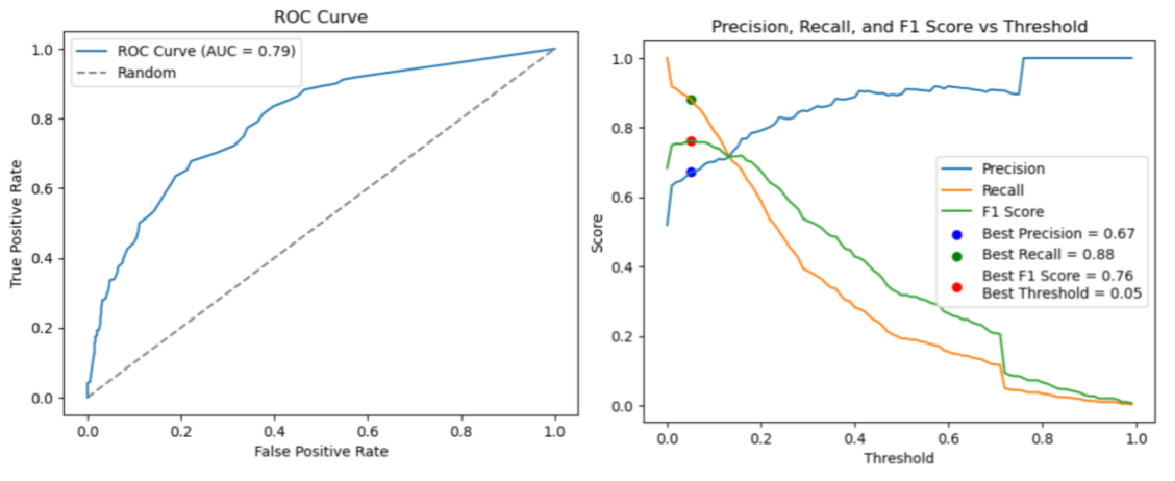
\includegraphics[width=1.0\linewidth]{./IPSJ202303_Ishioka/BoW_Program.pdf}
%	\caption{BoWでの結果(プログラムファイルのみ)}
%	\label{fig:oss_developments}
%\end{figure}
%%--------------------------------
%\begin{figure}[t]
% 	\centering
%		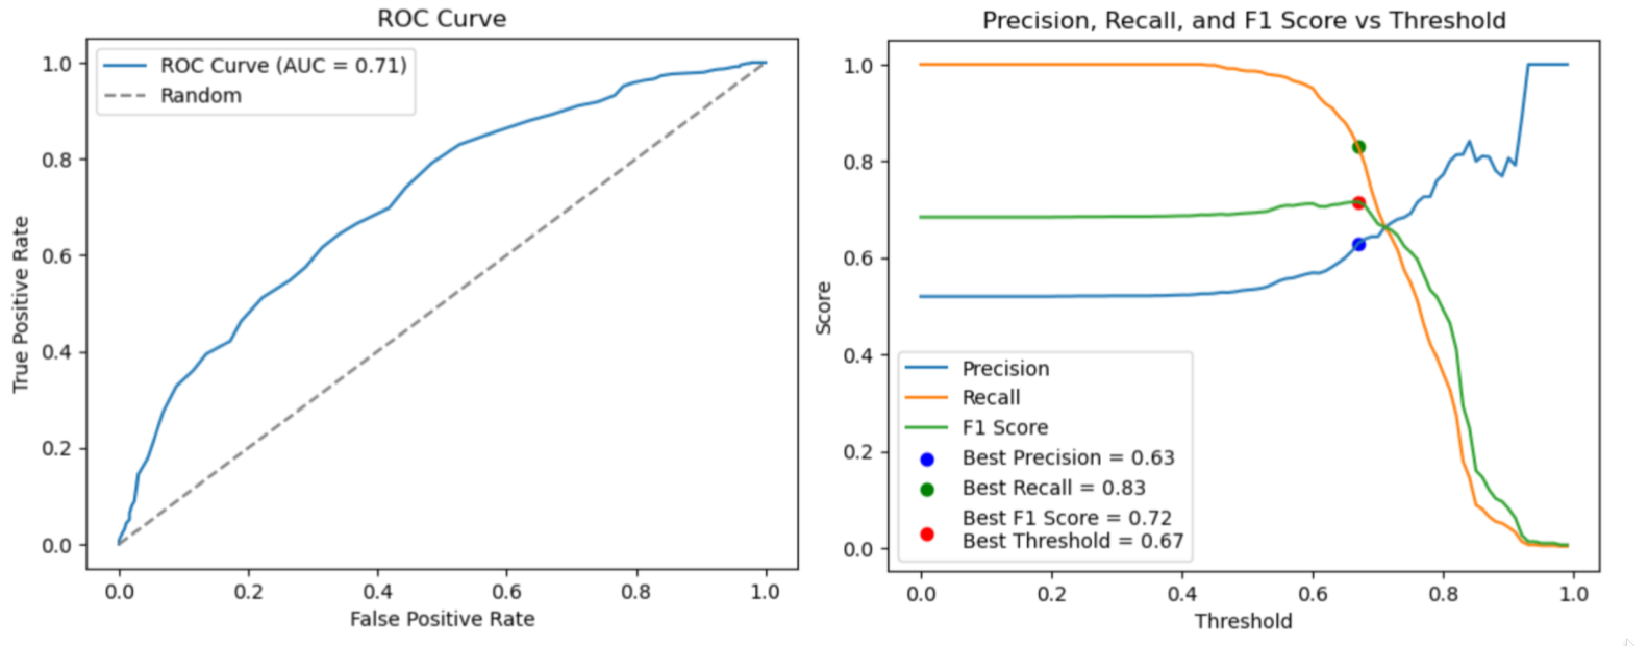
\includegraphics[width=1.0\linewidth]{./IPSJ202303_Ishioka/BERT_Program.pdf}
%	\caption{BERTでの結果(プログラムファイルのみ)}
%	\label{fig:oss_developments}
%\end{figure}
%%--------------------------------
%\begin{figure}[t]
% 	\centering
%		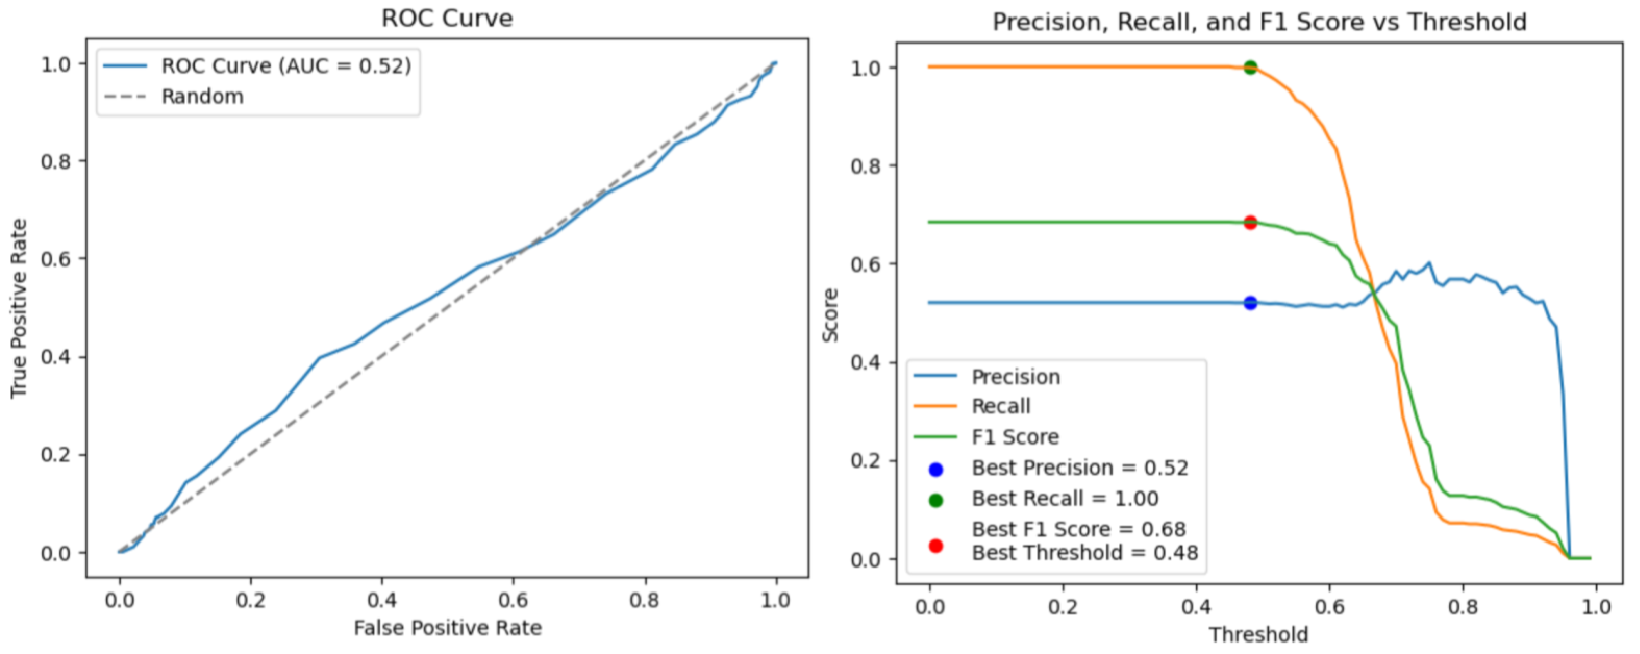
\includegraphics[width=1.0\linewidth]{./IPSJ202303_Ishioka/CodeBERT_Program.pdf}
%	\caption{CodeBERTでの結果(プログラムファイルのみ)}
%	\label{fig:oss_developments}
%\end{figure}
%%--------------------------------
%\begin{figure}[t]
% 	\centering
%		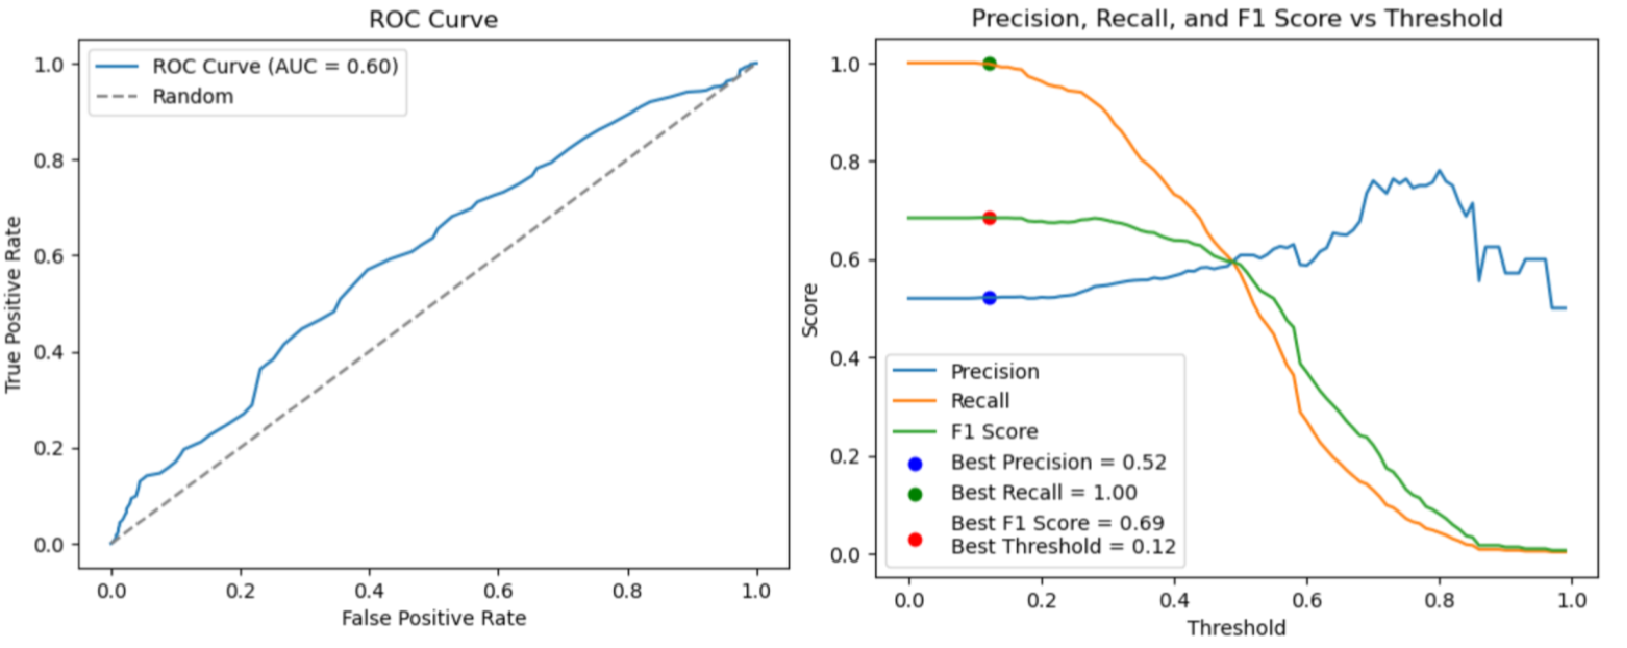
\includegraphics[width=1.0\linewidth]{./IPSJ202303_Ishioka/CodeT5_Program.pdf}
%	\caption{CodeT5+での結果(プログラムファイルのみ)}
%	\label{fig:oss_developments}
%\end{figure}
%%--------------------------------





%% 6章ーーーーーーーーーーーーーーーーーーーーーーーーーーーーーーーーーーーーーーーーーーーーーーーーーーー
\section{考察}
%% 6-1ーーーーーーーーーーーーーーーーーーーーーーーーーーーー
\subsection{分析1の考察}
本節では,4章で初期版READMEと最終版READMEを比較した結果を考察する.6.1.1では,一致率が高く,文字数が増えた項目を追加分析する.6.1.2では,初期版READMEには存在せず,最終版READMEにかけて追加された項目を追加分析する.

\subsubsection{文字数が増加する項目は何か}
図4.3の結果から,READMEの変更において,ソースコードの変更とは無関係な情報の移動は行われず,文章が追加されていくことが明らかとなった.一致率が高く,文字数が増えた項目を追加分析する.具体的には,図4.3における「追加」,つまり文章が初期版READMEと比べ増加している項目を明らかにした.表6.1は,初期版READMEと比べ最終版READMEで文字数が増加した上位5項目を示す.その結果は,使用方法,インストール方法,ライセンス,API,オプションの順で,文字数が初期版と比べ増加していることがわかった.これらの項目は,ソフトウェアの機能追加やAPI追加に伴って,利用者に新機能の使い方やAPIの詳細情報を伝えるために文章が追加されると考えられる.結果から,開発者はソフトウェアの利用方法やライセンスなどの,利用者にとって重要な情報を提供することに注力していることが示唆される.今後,READMEの項目ごとに,説明文の変更とファイルの変更を紐づけることで,開発者がファイルを変更する場合に,READMEの項目をどのように変更する必要があるのか推奨することができる.特に,利用者向けの項目(使用方法,インストール方法など)の説明文と紐づけることで,開発者のREADME変更を支援できると考える.


%\textcolor{red}{今後,}開発者がファイルを変更する場合に,利用者向けの項目(使用方法,インストール方法など)の説明文の変更と紐付けることで,\textcolor{red}{開発者がREADMEのどの項目を変更する必要があるのか推奨することで,}開発者のREADME変更を支援できると考えられる.


%開発者のREADME変更を支援する上で,既存の項目を変更する場合は,利用者向けの項目が変更される





%--------------------------------
%文字数が増えている項目
\begin{table}[t]
  \caption{文字数が増加した項目上位5件}
  \ecaption{hoge}
  \centering
  \begin{tabular}{l|r}
    \hline\hline
    項目 & 文字量が増加した\\
    & 項目数(37,648件)\\
    \hline
    その他       & 20,977 \\
    使用方法           & 6,603 \\
    インストール方法       & 3,535 \\
    ライセンス         & 1,758 \\
    API  & 1,421 \\
    オプション  & 650 \\
    \hline
  \end{tabular}
  \label{tab:file_comparison}
\end{table}
%--------------------------------


\subsubsection{追加される項目は何か}
表4.2で,初期版READMEから最終版READMEにかけて項目が追加されていることが明らかとなった.初期版READMEには存在せず,最終版READMEにかけて追加された項目を追加分析する.表6.2は,初期版READMEから最終版READMEにかけて追加された上位5項目を示す.その結果は,インストール方法,ライセンス,使用方法,貢献方法,APIの順で多く,これらの項目が追加されることがわかった.結果から,プロジェクトの成熟につれ,利用者向けの項目(使用方法,インストール方法など)だけでなく,開発者向けの項目(貢献方法,テストなど)が追加されると示唆される.今後,READMEの項目ごとに,説明文の変更とファイルの変更を紐づけることで,開発者がファイルを変更する場合に,READMEのどの項目を追加する必要があるのか推奨することができる.特に,開発者向けの項目(貢献方法,テストなど)の説明文と紐づけることで,開発者のREADME変更を支援できると考える.


%これらの項目は,ソフトウェアがある程度成熟してから記述する内容であり,利用者にとって重要なソフトウェアの使用方法などの項目だけでなく,外部の開発者や貢献者に向けたプロジェクトを拡大するための内容も追加されている.結果から,プロジェクトの成熟につれ,利用者向けの内容だけでなく,外部の開発者や貢献者に向けた内容が追加されると示唆される.プロジェクトの成熟につれ,利用者向けの項目(使用方法,インストール方法など)だけでなく,開発者向けの項目(貢献方法,テストなど)の説明文の変更とファイルに変更を紐付けることが有効であると考えられる.


%開発者のREADME変更を支援する上で,新規の項目を追加する場合は,利用者向けの項目だけでなく,貢献者向けの項目が追加される



%--------------------------------
%新しく追加された項目
\begin{table}[t]
  \caption{初期版READMEから最終版READMEにかけて追加された項目上位5件}
  \ecaption{hoge}
  \centering
  \begin{tabular}{l|r}
    \hline
    項目 & 項目追加数\\
    & (262,734件)\\
    \hline
    その他       & 167,044 \\
    使用方法           & 23,321 \\
    インストール方法       & 21,258 \\
    ライセンス         & 9,183 \\
    API  & 7,381 \\
    貢献方法  & 6,011 \\
    \hline
  \end{tabular}
  \label{tab:file_comparison}
\end{table}
%--------------------------------





%% 6-2ーーーーーーーーーーーーーーーーーーーーーーーーーーーー
\subsection{分析2の考察}
本節では,5章でREADMEとその他のファイルの紐付けを行った結果を考察する.BoW,BERT,CodeBERTの3つのモデルごとに紐付けられたファイルの違いを追加分析する.
図6.1は,モデルごとに共通して紐付けできたファイルの数を示す.結果から,BoW,BERT,CodeBERTの3つのモデルで共通して紐付けできたファイル数は81件,BoWのみで紐付けできたファイル数は18件,BERTのみで紐付けできたファイル数は1件,CodeBERTのみで紐付けできたファイル数は7件であった.
BoWのみで紐付けできたファイルを目視で確認した結果,依存関係の変更,関数の追加,機能の追加に伴うREADMEの変更があった.これらの変更には,関数名や機能の名前などのキーワードが複数回出現していたため,BoWのみで紐付けできたと考える.
BERTのみで紐付けできたファイルを目視で確認した結果,ファイルでは関数を追加し,関数追加に伴う機能の説明がREADMEに追加されるという変更であった.この変更では,関数名や機能の名前などのキーワードの出現が少なく,文脈を考慮することができたため,BERTのみで紐付けできたと考える.
CodeBERTのみで紐付けできたファイルを目視で確認した結果,関数の引数をコードを用いてREADMEに説明を加える変更,プログラムファイルでどのような変更をしたのか要約した文章をREADMEに追加する変更があった.これらの変更はプログラムの文脈を考慮することができたため,CodeBERTのみで紐付けできたと考える.





%各手法のみで取れたやつ 各手法のみでしか紐付けできないファイル数
%--------------------------------
\begin{figure}[t]
 	\centering
    		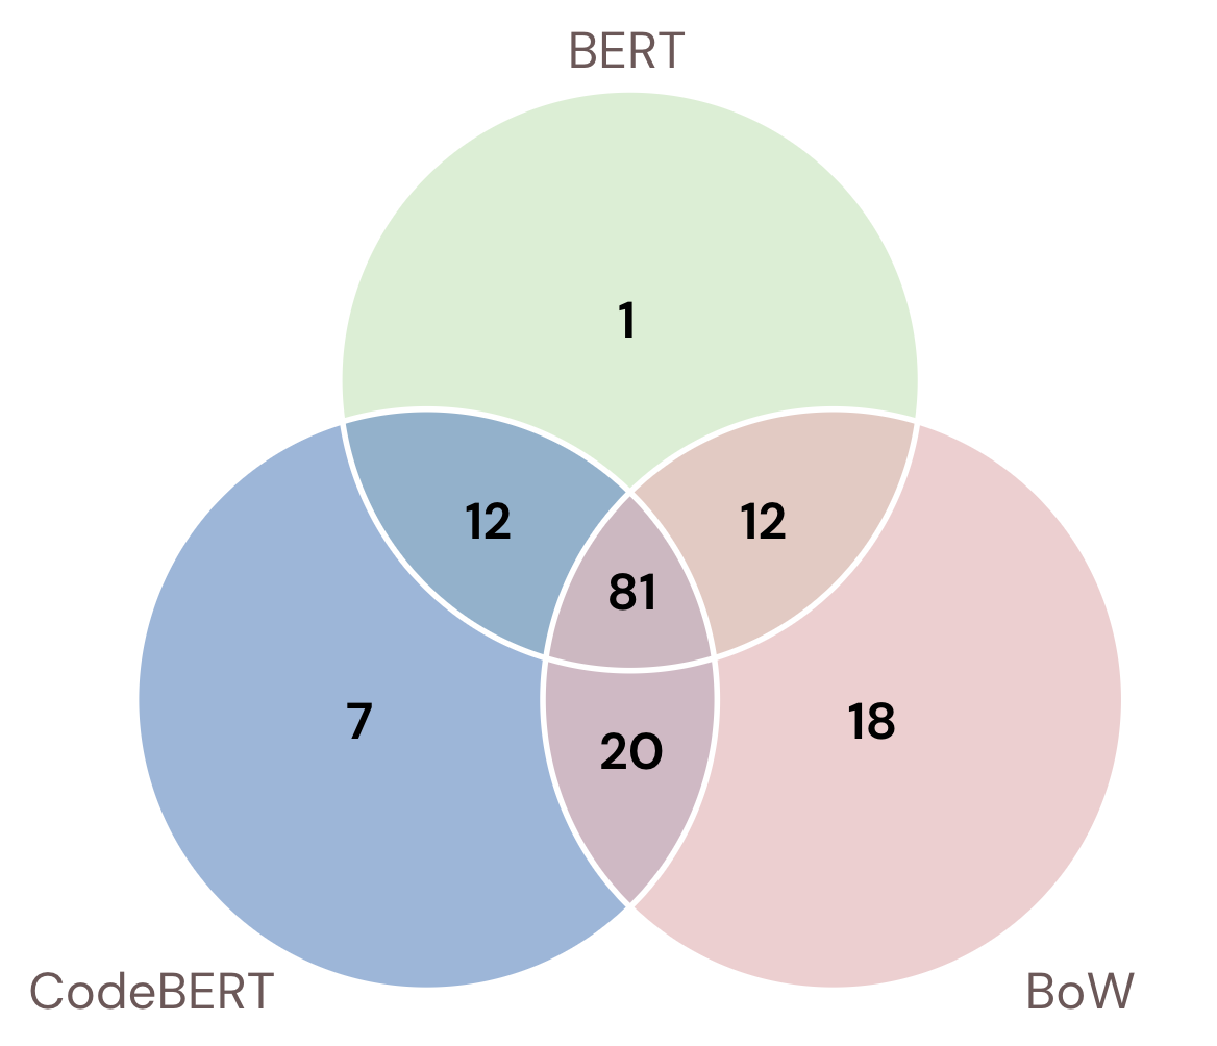
\includegraphics[width=0.8\linewidth]{./IPSJ202303_Ishioka/benz.pdf}
	\caption{モデルごとに共通して紐付けできたファイルの数}
        \ecaption{hoge}
	\label{fig:oss_developments}
\end{figure}
%--------------------------------









%\subsection{手法ごとで紐付けられたファイルの違い}
%5章では,READMEとその他のファイルの紐付けを機械的に行うために,BoW,BERT,CodeBERT,CodeT5+の4つの手法を用いて,変更差分の類似度を算出した.図5.1から図5.8のAUCの結果から,BoWとBERTのAUCが,プログラムを事前学習したCodeBERTとCodeT5+よりも性能が高いことが明らかとなった.各手法でしか紐付けができないファイルがあるのか追加分析を行った.表6.3は各手法でしか紐付けができなかったファイル数を示す.結果から,各手法でしか紐付けできないファイルは,CodeBERTの1件のみであった.このファイルはプログラムファイルで,その変更内容はソフトウェアの機能追加に関するもので,READMEの項目「使用方法」が変更されていた.
%
%また,プログラムを事前学習したCodeBERTとCodeT5+のみでしか紐付けができないファイルは31件存在した.表6.4にその内訳を示す.その結果,「js」や「json」ファイルなどのプログラムファイルを紐付けできていた.その変更内容はソフトウェアの機能追加に関するものや依存関係の変更に関するもの,関数の追加に関する変更などがあった.図5.1から図5.8のAUCの結果から,CodeBERTとCodeT5+は,BoWとBERTのAUCの値を下回る一方で,ソフトウェアの機能追加や関数追加などのプログラムを事前学習したからこそ紐付けが可能となったファイルが存在する.そのため,READMEとその他のファイルの紐付けを行う上で,プログラムを事前学習させたモデルを用いることは有用であると言える.







%%各手法のみで取れたやつ 各手法のみでしか紐付けできないファイル数
%\begin{table}[H]
%  \caption{各手法独自に紐付け可能なファイル数}
%  \centering
%  \begin{tabular}{l|r}
%    \hline
%    \textbf{ベクトル化手法} & \textbf{紐付けファイル数}\\
%    & \textbf{(781件)}\\
%    \hline
%    BoWのみ       & 0件 \\
%    BERTのみ           & 0件 \\
%    CodeBERTのみ       & 1件 \\
%    CodeT5+のみ         & 0件 \\    
%    \hline
%    BoWとBERTのみ         & 0件 \\
%    CodeBERTとCodeT5+のみ         & 31件 \\
%    \hline
%  \end{tabular}
%  \label{tab:file_comparison}
%\end{table}
%
%
%%コードモデルのみで取れたやつ
%\begin{table}[H]
%  \caption{プログラムを事前学習した手法のみで紐付けできたファイル}
%  \centering
%  \begin{tabular}{l|r}
%    \hline
%    \textbf{拡張子名} & \textbf{CodeBERTとCodeT5+のみで}\\
%    & \textbf{紐付けできた数(31件)}\\
%    \hline
%    js       & 14件 \\
%    json           & 6件 \\
%    yml       & 2件 \\
%    css         & 2件 \\    
%    LICENSE         & 1件 \\    
%    ts         & 1件 \\    
%    vue         & 1件 \\    
%    md         & 1件 \\    
%    txt         & 1件 \\    
%    lock         & 1件 \\    
%    scss         & 1件 \\    
%    \hline
%  \end{tabular}
%  \label{tab:file_comparison}
%\end{table}





%なぜP考慮モデルの性能が上がらなかったのか,どうすれば改善できそうか
%どんな項目がファイルとともに更新されているのか→XXXXの項目→XXXXの項目はXXXの特徴がある,だからPモデルの性能が上がらなかったのでは??
%RMには1行だけ,他ファイルはたくさん更新の例 → RMとファイルを完全に紐付けるのは難しい...


%どういう目的で変更されたか(変更意図は??)→リネームや新規の追加が多かった.


%各手法で取れたやつ取れなかったやつの違いは?かぶりはある?Pファイルの割合は??→そもそもファイルの類似低い?,RMが自然言語で書かれる&書き方多様であるため,紐付けが難しい??





%% 6-3ーーーーーーーーーーーーーーーーーーーーーーーーーーーー
\subsection{妥当性の脅威}
\subsubsection{内的妥当性}
READMEおよびその他のファイルの変更差分の分散表現を得るために用いたベクトル化手法について議論する.本論文では,BoW,BERT,CodeBERTを使用したが,使用するベクトル化手法によって評価結果に違いが生じる可能性がある.しかし,本論文では,文脈を考慮していないBoW,事前学習されたモデルで文脈を考慮したBERT,複数のプログラムで事前学習されたモデルのCodeBERTを使用することでその脅威を削減する.

正解データセット作成について議論する.本論文では,READMEおよびその他のファイルの変更意図が一致するのか否かを,著者が目視によって分類している.著者は一定のソフトウェア開発の知識を有するが,READMEおよびその他のファイルのすべての変更内容を把握して分類することは難しく,誤って分類している可能性がある.しかし,目視による分類は著者と共同研究者間で合意を形成することで行っており,その脅威を削減する.

%また,目視による分類は信頼区間を考慮しているため,本論文の結果は妥当であるといえる.


READMEとその他のファイルの紐付け手法について議論する.本論文では,紐付けを行うために,同時に変更されたREADMEおよびその他のファイルの変更差分に着目した.READMEとその他のファイルの紐付けを行う手法として,コミットメッセージの利用やREADME変更前後のコミットで変更されたファイル変更を利用することで,新たな知見を得られることが考えられる.しかし,READMEとその他のファイルの紐付け手法について,従来研究では明らかにされていないため,本論文により十分な知見を得ることができたと考える.



%%ーーーーーーーーーーーーーーー
\subsubsection{外的妥当性}
正解データセット作成について議論する.本論文では,正解データセット作成の際,対象コミットのすべてを目視で調査したわけではない.しかし,目視対象とするデータは信頼区間95\%,信頼区間±5\%でランダムにサンプリングしているため,結果は一般化できる.


対象プロジェクトについて議論する.本論文では,JavaScript言語を使用するプロジェクトのREADMEを対象としている.本論文の手法は,MarkDown形式で記述し,見出し機能を使用しているREADMEであれば,同様に実行できるため,JavaScript以外の言語を使用するプロジェクトにおけるREADMEを対象とした場合でも同様の結果が得られると考える.別言語で開発されたプロジェクトのREADMEを対象とすることで,言語間での手法の有用性の違いなどの新たな知見が得られると考える.







%% 7章ーーーーーーーーーーーーーーーーーーーーーーーーーーーーーーーーーーーーーーーーーーーーーーーーーーー
\section{おわりに}
本論文では,開発者のREAME変更支援のために,同時に変更されるREADMEとその他のファイルの紐付け手法の提案を行った.分析1では,READMEをどのように変更するのかを明らかにするために,52,292件のプロジェクトを対象に,初期版READMEと最終版READMEの項目と説明文を比較した.その結果,READMEの変更において,ソースコードの変更とは無関係なREADMEの変更が行われる可能性は低く,ソースコードの変更とともに項目ごとに情報を追加していくことを明らかにした.具体的には,ソフトウェアの変更に伴って,使用方法やインストール方法,ライセンス,APIといった項目を追加し,説明文に文章を追加していくことを明らかにした.

分析2では,提案手法によってREADMEの変更とその他のファイルの変更を機械的に紐付けることができるのかを調査した.同時に変更されたREADMEの変更内容とファイルの変更内容を入力として,READMEとファイルの変更意図が一致するか否かの2クラス分類を行い,3つのモデル(BoW,BERT,CodeBERT)で比較した.その結果,CodeBERT(F1値=0.81),BoW(F1値=0.78),BERT(F1値=0.77)の順で高く,READMEとファイルの紐付けにおいて,CodeBERTモデルが適合率と再現率の両方で良好な性能を示した.

本論文で提案するREADMEとその他のファイルの紐付け手法は,開発者のファイル変更に合わせて,README変更を開発者に推薦することで,開発者のREADME変更支援やREADMEを常に最新の状態にするといったREADMEの品質向上につながることを期待する.

今後の発展として,対象とする言語を増やし,より一般的な結果を得ることが挙げられる.また,README変更前後のコミットで変更されたファイル変更との紐付けにより,より詳細な開発者へのREADME変更の推薦を行うことが挙げられる.また,READMEとその他のファイルの紐付け手法として変更差分以外の情報を利用することで,より正確な紐付けを行うことが考えられる.



\bibliographystyle{ipsjunsrt}
\bibliography{bibfile_IPSJjournal_ishioka}

\begin{biography}
\profile{n}{石岡 直樹}{2024年和歌山大学システム工学研究科在学中,ソフトウェア工学,特にソフトウェアドキュメント生成の研究に従事.}
%
\profile{m}{伊原 彰紀}{2009年奈良先端科学技術大学院大学情報科学研究科博士前期課程修了.2012年同大学博士後期課程修了.2012年同大学情報科学研究科助教.2018年和歌山大学システム工学部講師.博士(工学).ソフトウェア工学,特にオープンソースソフトウェア開発・利用支援の研究に従事.電子情報通信学会,IEEE各会員.}

\end{biography}



\end{document}
